%% ============================================================================
%%  CAPITOLO 10 — La formula di Taylor
%%  Fonte principale per argomenti e dimostrazioni: Marcellini–Sbordone, cap. 10
%%  (§77 resto di Peano, o piccolo, sviluppi delle funzioni elementari; §78 uso
%%  della formula di Taylor nel calcolo di limiti, proprietà degli o piccoli;
%%  §79 resto integrale; §80 resto di Lagrange; appendice: §81 tabulazione di
%%  funzioni, stima del resto).
%% ============================================================================
\aperturacapitolo{La formula di Taylor}{cap:taylor}

\epigraph{Théorie des fonctions analytiques, contenant les principes du calcul
différentiel, dégagés de toute considération d'infiniment petits ou d'évanouissans, de
limites ou de fluxions, et réduits à l'analyse algébrique des quantités finies.\\[2pt]
\upshape(Teoria delle funzioni analitiche, contenente i principi del calcolo
differenziale, liberati da ogni considerazione di infinitamente piccoli o di quantità
evanescenti, di limiti o di flussioni, e ridotti all'analisi algebrica delle quantità
finite.)}{Joseph-Louis Lagrange, frontespizio della \emph{Théorie des fonctions
analytiques} (1797)}

\lettrine[lines=3, findent=2pt, nindent=0pt]{L}{a formula di Taylor} con il resto di
Peano è stata introdotta nel \cref{sec:taylor}, dove ne abbiamo visto le prime
conseguenze: gli sviluppi delle funzioni elementari, il calcolo di qualche limite, le
approssimazioni per piccoli angoli e il criterio per i punti di massimo e di minimo
basato sulle derivate successive. In questo capitolo la riprendiamo e la completiamo in
tre direzioni.

La prima è \emph{operativa}: impariamo a manipolare gli «o piccoli» con regole precise,
che rendono la formula di Taylor lo strumento più potente per il calcolo dei limiti, e
a ottenere nuovi sviluppi senza calcolare derivate, componendo e integrando quelli già
noti. La seconda è \emph{quantitativa}: il resto di Peano dice che l'errore è
trascurabile vicino al punto iniziale, ma non quanto vale; il resto in forma integrale e
quello nella forma di Lagrange, ricavati con il calcolo integrale, permettono di
\emph{stimarlo}. La terza è \emph{numerica}: con queste stime si calcolano le funzioni
elementari con precisione prefissata, come facevano i compilatori delle tavole dei
logaritmi e come fanno, con metodi più raffinati, i computer di bordo. Lungo la
strada calcoleremo la distanza dell'orizzonte vista da un velivolo, le cifre di $\pi$ con
la formula di Machin, e dimostreremo che il numero $e$ è irrazionale. Seguiremo il testo
di riferimento \cite{marcellini-sbordone}.

\medskip
\noindent\textbf{In questo capitolo.}
\begin{itemize}
  \item Il resto di Peano; polinomi e loro sviluppi; nuovi sviluppi per composizione e
  per integrazione; lo sviluppo dell'arcotangente (\S\ref{sec:taylor-peano}).
  \item L'algebra degli o piccoli e il calcolo dei limiti (\S\ref{sec:o-piccoli}).
  \item Il resto integrale (\S\ref{sec:resto-integrale}) e il resto di Lagrange
  (\S\ref{sec:resto-lagrange}).
  \item Approfondimento: la forma di Cauchy del resto (\S\ref{subsec:resto-cauchy}).
  \item Appendice: stima del resto, tabulazione, irrazionalità di $e$
  (\S\ref{sec:tabulazione}); approfondimento: una tavola dei logaritmi
  (\S\ref{subsec:tavola-logaritmi}).
  \item Esercizi di riepilogo (\S\ref{sec:esercizi-cap10}).
  \item Punti fondamentali del capitolo (\S\ref{sec:sintesi-cap10}).
\end{itemize}

%% ----------------------------------------------------------------------------
%%  §10.1  Il resto di Peano. Nuovi sviluppi
%% ----------------------------------------------------------------------------
\section{Il resto di Peano}
\label{sec:taylor-peano}

\subsection{Polinomi e loro sviluppi}

Consideriamo un polinomio di grado $n$ a coefficienti reali,
$p(x)=a_{0}+a_{1}x+a_{2}x^{2}+\dots+a_{n}x^{n}$. La funzione $p$ è derivabile infinite volte in
$\R$, le sue derivate di ordine maggiore di $n$ sono tutte nulle, e, come nella
dimostrazione del \cref{lem:derivate-taylor}, $p^{(k)}(0)=k!\,a_{k}$ per ogni $k\le n$.
Ricavando i coefficienti, il polinomio si scrive
\begin{equation}\label{eq:polinomio-mac-laurin}
  p(x)=p(0)+\frac{p'(0)}{1!}\,x+\frac{p''(0)}{2!}\,x^{2}+\dots+\frac{p^{(n)}(0)}{n!}\,x^{n} :
\end{equation}
un polinomio di grado $n$ è noto una volta noti il suo valore e quelli delle sue prime
$n$ derivate nello zero. Lo stesso vale per un qualsiasi punto $x_{0}$.

\begin{proposizione}[Un polinomio coincide con il proprio sviluppo]
\label{prop:polinomio-sviluppo}
Sia $p$ un polinomio di grado $\le n$ e sia $x_{0}\in\R$. Allora
\begin{equation}\label{eq:polinomio-sviluppo}
  p(x)=\sum_{k=0}^{n}\frac{p^{(k)}(x_{0})}{k!}\,(x-x_{0})^{k} \qquad\perogni x\in\R .
\end{equation}
In particolare, un polinomio di grado $\le n$ è univocamente determinato dai valori che
esso e le sue prime $n$ derivate assumono in $x_{0}$.
\end{proposizione}

\begin{schema}
\Ipotesi{$p$ polinomio di grado $\le n$; \ $x_{0}\in\R$.}
\Tesi{$p(x)=\sum_{k=0}^{n}\frac{p^{(k)}(x_{0})}{k!}(x-x_{0})^{k}$ per ogni $x$: il resto della formula di
Taylor di ordine $n$ è identicamente nullo.}
\end{schema}

\begin{strategia}
Si cambia variabile ponendo $h=x-x_{0}$: il polinomio $q(h)=p(x_{0}+h)$, sviluppati i
binomi, è un polinomio di grado $\le n$ in $h$, e per esso vale la
\eqref{eq:polinomio-mac-laurin}. Resta da osservare che le derivate di $q$ in $0$ sono quelle
di $p$ in $x_{0}$.
\end{strategia}

\begin{dimostrazione}
Sia $q(h)=p(x_{0}+h)$. Sviluppando ciascuna potenza $(x_{0}+h)^{j}$ con la formula del binomio
(\cref{teo:binomio}) e raccogliendo, $q$ è un polinomio di grado $\le n$ nella variabile
$h$, diciamo $q(h)=\sum_{k=0}^{n}c_{k}h^{k}$, e quindi $c_{k}=\frac{q^{(k)}(0)}{k!}$. Per la regola di
derivazione delle funzioni composte (con la funzione interna $h\mapsto x_{0}+h$, di derivata
$1$), $q^{(k)}(h)=p^{(k)}(x_{0}+h)$, e in particolare $q^{(k)}(0)=p^{(k)}(x_{0})$. Dunque
$p(x)=q(x-x_{0})=\sum_{k=0}^{n}\frac{p^{(k)}(x_{0})}{k!}(x-x_{0})^{k}$. L'ultima affermazione segue
perché il secondo membro dipende soltanto dai numeri $p^{(k)}(x_{0})$.
\end{dimostrazione}

Ad esempio, il polinomio $p(x)=x^{3}$ ha in $x_{0}=1$ le derivate $p(1)=1$, $p'(1)=3$,
$p''(1)=6$, $p'''(1)=6$, e quindi $x^{3}=1+3(x-1)+3(x-1)^{2}+(x-1)^{3}$, come si verifica
anche con la formula del binomio applicata a $\bigl(1+(x-1)\bigr)^{3}$.

\begin{notastorica}[Taylor, Mac Laurin e le differenze finite]
Taylor arrivò al suo sviluppo partendo da un analogo «discreto» della
\cref{prop:polinomio-sviluppo}. Fissato un passo $h$, le \emph{differenze in avanti}
$\Delta f(x_{0})=f(x_{0}+h)-f(x_{0})$, $\Delta^{2}f(x_{0})=\Delta f(x_{0}+h)-\Delta f(x_{0})$, \dots\
ricostruiscono i valori di $f$ nei punti $x_{0}+mh$ mediante la formula di interpolazione
di Newton (\emph{Principia}, 1687, già in una lettera di James Gregory del 1670):
\[
\begin{aligned}
  f(x_{0}+mh)&=\sum_{k=0}^{m}\binom mk\Delta^{k}f(x_{0})\\
  &=\sum_{k=0}^{m}\frac{v(v-h)\cdots\bigl(v-(k-1)h\bigr)}{k!}\cdot\frac{\Delta^{k}f(x_{0})}{h^{k}} ,
\end{aligned}
\]
dove $v=mh$. Taylor, che annunciò il teorema in una lettera del 26 luglio 1712 a John
Machin (lo stesso della formula \eqref{eq:machin}), fissò $v=x-x_{0}$ e lasciò «svanire»
gli incrementi: per $h\to0$ il primo fattore diventa $\frac{(x-x_{0})^{k}}{k!}$ e il secondo la
flussione, cioè la derivata $f^{(k)}(x_{0})$. Ecco l'origine dei coefficienti
$\frac{f^{(k)}(x_{0})}{k!}$; ma il passaggio al limite non era giustificato, perché il numero
dei termini cresce con $m$. Mac Laurin, nel \emph{Treatise of Fluxions} (1742), scritto per
rispondere alle critiche di Berkeley (\S\ref{sec:def-limite}), seguì un'altra strada:
supposto $f(x)=A+Bx+Cx^{2}+\cdots$, derivò ripetutamente e pose $x=0$, esattamente come
per la \eqref{eq:polinomio-mac-laurin}, riconoscendo che la formula era un caso
particolare di quella di Taylor; essa compariva già nel \emph{Methodus differentialis}
(1730) di James Stirling. Né Taylor né Mac Laurin si chiesero quanto valesse l'errore
commesso arrestando la somma: è la domanda a cui risponde questo capitolo.
\end{notastorica}

Sia ora $f$ una funzione derivabile $n$ volte in un punto $x_{0}$ (nel senso della
\cref{not:derivabile-n-volte}). Per la \cref{prop:polinomio-sviluppo}, il polinomio di
grado $\le n$ che ha nel punto $x_{0}$ lo stesso valore e le stesse prime $n$ derivate di
$f$ esiste, è unico, ed è il polinomio di Taylor $T_{n}$ della
\eqref{eq:polinomio-taylor}. La funzione $R_{n}(x)=f(x)-T_{n}(x)$, il \emph{resto}, rappresenta
l'errore che si commette sostituendo a $f(x)$ il suo polinomio di Taylor, e il
\cref{teo:taylor} afferma che
\begin{equation}\label{eq:peano-richiamo}
  f(x)=\sum_{k=0}^{n}\frac{f^{(k)}(x_{0})}{k!}(x-x_{0})^{k}+o\bigl((x-x_{0})^{n}\bigr)
  \qquad (x\to x_{0}) .
\end{equation}
Ricordiamo che la dimostrazione data nel \cref{sec:taylor} richiede soltanto l'esistenza
di $f^{(n)}(x_{0})$, e non la continuità di $f^{(n)}$ in $x_{0}$. Ad esempio, la funzione
$f(x)=x^{4}\sen\frac1x$, prolungata con $f(0)=0$, ha $f'(0)=f''(0)=0$, ma $f''$ non è continua
in $0$ (per $x\neq0$ contiene il termine $-\sen\frac1x$, che oscilla); la formula di Taylor di
ordine $2$ dice che $f(x)=o(x^{2})$, come è evidente da $\abs{f(x)}\le x^{4}$.

\subsection{Nuovi sviluppi senza calcolare derivate}

Calcolare le derivate successive di una funzione composta è in genere laborioso. Per la
\cref{prop:unicita-taylor}, però, \emph{qualunque} procedimento produca un polinomio di grado
$\le n$ che approssima $f$ con un errore $o\bigl((x-x_{0})^{n}\bigr)$ fornisce il polinomio di
Taylor. I due procedimenti più utili sono la sostituzione e l'integrazione.

\begin{lemma}[Sostituzione negli o piccoli]\label{lem:sostituzione-o}
Sia $g(t)=o(t^{m})$ per $t\to0$, e sia $\varphi$ una funzione con $\varphi(x)\to0$ per $x\to x_{0}$ e
$\varphi(x)\neq0$ per $x\neq x_{0}$. Allora $g\bigl(\varphi(x)\bigr)=o\bigl(\varphi(x)^{m}\bigr)$ per $x\to x_{0}$.
\end{lemma}

\begin{schema}
\Ipotesi{$\frac{g(t)}{t^{m}}\to0$ per $t\to0$; \ $\varphi(x)\to0$, $\varphi(x)\neq0$ per $x\neq x_{0}$.}
\Tesi{$\frac{g(\varphi(x))}{\varphi(x)^{m}}\to0$ per $x\to x_{0}$.}
\end{schema}

\begin{strategia}
Il rapporto $\frac{g(\varphi(x))}{\varphi(x)^{m}}$ è la funzione $\frac{g(t)}{t^{m}}$ calcolata in $t=\varphi(x)$: è il
teorema sul limite delle funzioni composte.
\end{strategia}

\begin{dimostrazione}
Posto $h(t)=\frac{g(t)}{t^{m}}$ per $t\neq0$, si ha $h(t)\to0$ per $t\to0$, e
$\frac{g(\varphi(x))}{\varphi(x)^{m}}=h(\varphi(x))$, con $\varphi(x)\to0$ e $\varphi(x)\neq0$ per $x\neq x_{0}$. Per il
teorema sul limite delle funzioni composte (\cref{teo:limite-composta}), $h(\varphi(x))\to0$.
\end{dimostrazione}

Ad esempio, da $\sen t=t-\frac{t^{3}}6+o(t^{4})$ \eqref{eq:taylor-sen}, con $t=x^{2}$ e $t=x^{3}$ si
ottiene
\begin{equation}\label{eq:sen-x2-x3}
  \sen x^{2}=x^{2}-\frac{x^{6}}6+o(x^{8}), \qquad \sen x^{3}=x^{3}-\frac{x^{9}}6+o(x^{12}) ,
\end{equation}
e in particolare $\sen x^{2}=x^{2}+o(x^{4})$ e $\sen x^{3}=x^{3}+o(x^{6})$: vicino a $0$ le funzioni
$\sen x^{2}$ e $\sen x^{3}$ hanno un «comportamento» simile a quello di $x^{2}$ e di $x^{3}$
(\cref{fig:taylor-composte}). Allo stesso modo, con $e^{x}-1=x+\frac{x^{2}}2+\frac{x^{3}}6+o(x^{3})$ e
$\sen u=u-\frac{u^{3}}6+o(u^{3})$, si trova
\[
  1+\sen\bigl(e^{x}-1\bigr)=1+x+\frac{x^{2}}2+o(x^{3}) ,
\]
perché il termine $\frac{x^{3}}6$ dello sviluppo di $e^{x}-1$ si elide con il $-\frac{u^{3}}6=-\frac{x^{3}}6+o(x^{3})$
del seno (le regole di calcolo degli o piccoli che stiamo usando saranno giustificate nel
\cref{sec:o-piccoli}): la funzione $1+\sen(e^{x}-1)$ ha in $0$ lo stesso polinomio di Taylor di ordine $2$
di $e^{x}$, e i due grafici sono simili vicino all'origine, mentre lontano da essa si
comportano in modo completamente diverso.

\begin{figure}[htb]
\centering
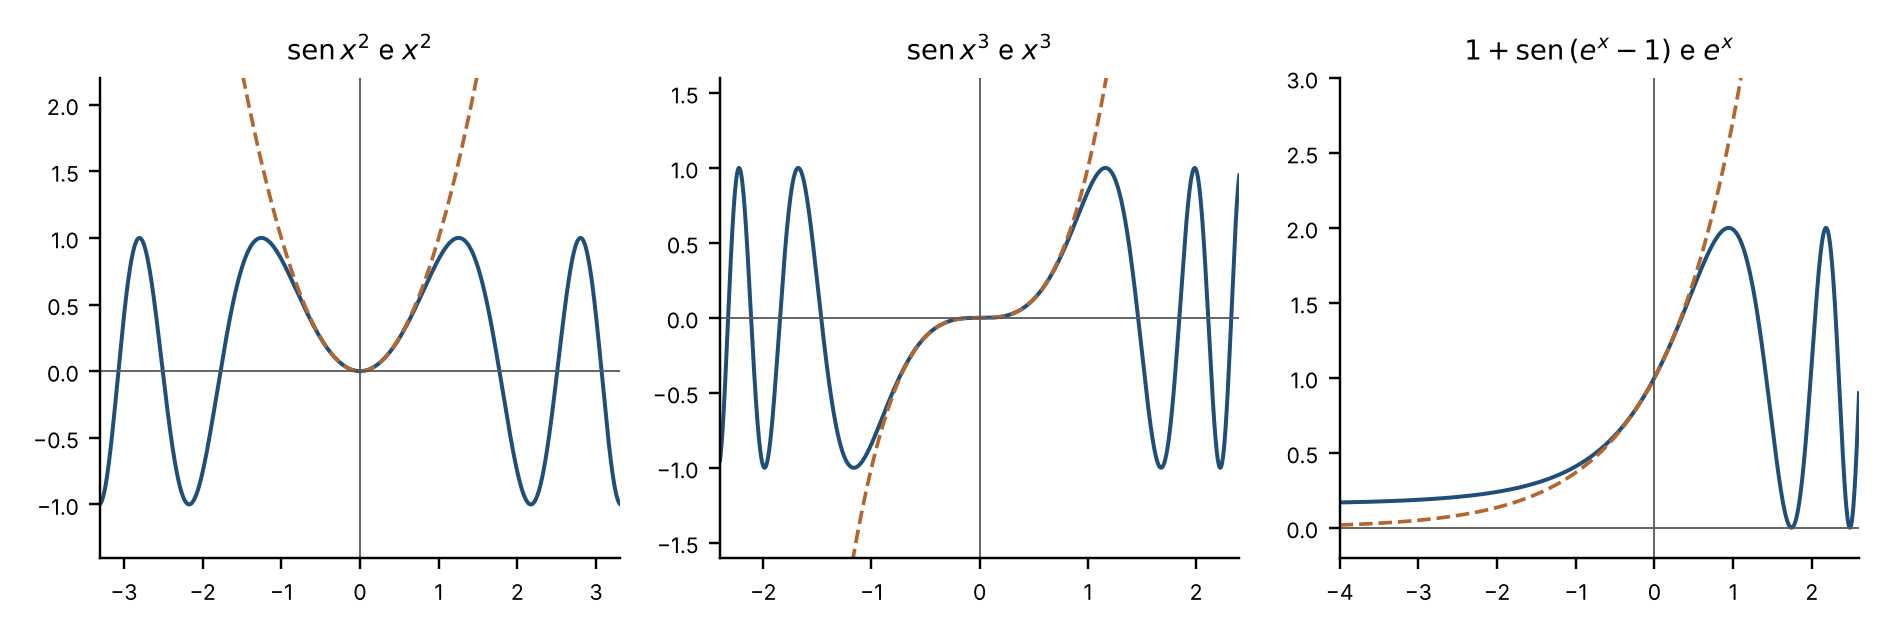
\includegraphics[width=\textwidth]{figure/taylor_composte.png}
\caption{Le funzioni $\sen x^{2}$, $\sen x^{3}$ e $1+\sen(e^{x}-1)$ (in blu) e le loro approssimazioni
vicino all'origine $x^{2}$, $x^{3}$, $e^{x}$ (tratteggio rame). Lontano dall'origine la
somiglianza scompare: $\sen x^{2}$ e $\sen x^{3}$ oscillano sempre più rapidamente, e
$1+\sen(e^{x}-1)$ oscilla per $x\to+\infty$ mentre tende a $1+\sen(-1)>0$ per $x\to-\infty$
(\texttt{python/fig\_taylor\_composte.py}).}
\label{fig:taylor-composte}
\end{figure}

Il secondo procedimento consiste nell'integrare uno sviluppo noto.

\begin{lemma}[Integrazione degli o piccoli]\label{lem:integrazione-o}
Sia $m\ge0$ un intero, e sia $g$ continua in un intorno $I$ di $0$, con $g(t)=o(t^{m})$ per
$t\to0$. Allora
\begin{equation}\label{eq:integrazione-o}
  \int_{0}^{x}g(t)\,dt=o(x^{m+1}) \qquad (x\to0) .
\end{equation}
\end{lemma}

\begin{schema}
\Ipotesi{$m\ge0$ intero; \ $g$ continua in $I\ni0$; \ $\frac{g(t)}{t^{m}}\to0$ per $t\to0$.}
\Tesi{$\frac1{x^{m+1}}\int_{0}^{x}g(t)\,dt\to0$ per $x\to0$.}
\end{schema}

\begin{strategia}
Vicino a $0$ si ha $\abs{g(t)}\le\epsilon\abs t^{m}$; integrando la disuguaglianza tra $0$ e $x$ si
ottiene una stima con $\frac{\epsilon\abs x^{m+1}}{m+1}$.
\end{strategia}

\begin{dimostrazione}
Sia $\epsilon>0$. Per l'ipotesi esiste $\delta>0$, che possiamo scegliere in modo che
$(-\delta,\delta)\subseteq I$, tale che $\abs{g(t)}\le\epsilon\abs t^{m}$ per $\abs t<\delta$
(anche per $t=0$, perché $g(0)=\lim_{t\to0}g(t)=0$ per la continuità). Per $0<\abs x<\delta$, per il
\cref{teo:valore-assoluto} e il confronto, applicati nell'intervallo di estremi $0$ e $x$,
\[
  \Bigl|\int_{0}^{x}g(t)\,dt\Bigr|\le\Bigl|\int_{0}^{x}\epsilon\abs t^{m}\,dt\Bigr|=\frac{\epsilon\abs x^{m+1}}{m+1}\le\epsilon\abs x^{m+1} ,
\]
cioè $\Bigl|\frac1{x^{m+1}}\int_{0}^{x}g\Bigr|\le\epsilon$, che è la tesi.
\end{dimostrazione}

Ne segue che uno sviluppo della derivata si può integrare «termine a termine»: se $f'$ è
continua vicino a $0$ e $f'(x)=\sum_{k=0}^{n}a_{k}x^{k}+o(x^{n})$, allora, per la formula
fondamentale e il lemma,
\begin{equation}\label{eq:integrazione-termine}
  f(x)=f(0)+\int_{0}^{x}f'(t)\,dt=f(0)+\sum_{k=0}^{n}\frac{a_{k}}{k+1}\,x^{k+1}+o(x^{n+1}) .
\end{equation}
Il procedimento inverso, cioè derivare uno sviluppo termine a termine, non è lecito in
generale: $x^{3}\sen\frac1x=o(x^{2})$, ma la sua derivata $3x^{2}\sen\frac1x-x\cos\frac1x$ non è $o(x)$.

\subsection{Lo sviluppo dell'arcotangente}

Applichiamo l'idea dell'integrazione all'arcotangente, le cui derivate successive sono
sempre più complicate. Il punto di partenza è che la sua derivata $\frac1{1+t^{2}}$ è la somma
di una progressione geometrica di ragione $-t^{2}$, a meno di un resto esplicito; in questo
modo otteniamo non soltanto lo sviluppo, ma anche una stima del resto valida per
\emph{ogni} $x$.

\begin{proposizione}[Sviluppo dell'arcotangente]\label{prop:sviluppo-arctg}
Per ogni $n\in\N\cup\set0$ e ogni $x\in\R$,
\begin{equation}\label{eq:sviluppo-arctg}
\begin{gathered}
  \operatorname{arctg}x=x-\frac{x^{3}}3+\frac{x^{5}}5-\dots+(-1)^{n}\frac{x^{2n+1}}{2n+1}+R(x),\\
  R(x)=(-1)^{n+1}\int_{0}^{x}\frac{t^{2n+2}}{1+t^{2}}\,dt, \qquad
  \abs{R(x)}\le\frac{\abs x^{2n+3}}{2n+3} .
\end{gathered}
\end{equation}
In particolare $R(x)=o(x^{2n+2})$ per $x\to0$, e il polinomio a secondo membro è il polinomio
di Taylor di ordine $2n+2$ dell'arcotangente in $0$.
\end{proposizione}

\begin{schema}
\Ipotesi{$n\ge0$ intero; \ $x\in\R$.}
\Tesi{la \eqref{eq:sviluppo-arctg}, con il resto in forma integrale e
$\abs{R(x)}\le\frac{\abs x^{2n+3}}{2n+3}$; \ $R(x)=o(x^{2n+2})$.}
\end{schema}

\begin{strategia}
La somma della progressione geometrica $1-t^{2}+t^{4}-\dots+(-1)^{n}t^{2n}$ è
$\frac{1-(-t^{2})^{n+1}}{1+t^{2}}$: dunque $\frac1{1+t^{2}}$ è uguale a questa somma più il resto esplicito
$\frac{(-1)^{n+1}t^{2n+2}}{1+t^{2}}$. Integrando tra $0$ e $x$, la somma dà il polinomio e il resto si
stima con $t^{2n+2}$, perché $1+t^{2}\ge1$. L'unicità del polinomio di Taylor fa il resto.
\end{strategia}

\begin{dimostrazione}
Per la formula della somma della progressione geometrica (\cref{prop:geometrica}) con
ragione $-t^{2}\neq1$,
\[
  \sum_{k=0}^{n}(-t^{2})^{k}=\frac{1-(-t^{2})^{n+1}}{1+t^{2}} ,
\]
cioè
\[
  \frac1{1+t^{2}}=\sum_{k=0}^{n}(-1)^{k}t^{2k}+(-1)^{n+1}\frac{t^{2n+2}}{1+t^{2}} .
\]
Integriamo tra $0$ e $x$: per la formula fondamentale, poiché $D\operatorname{arctg}t=\frac1{1+t^{2}}$
\eqref{eq:derivata-arctg} e $\operatorname{arctg}0=0$,
\[
  \operatorname{arctg}x=\sum_{k=0}^{n}(-1)^{k}\frac{x^{2k+1}}{2k+1}+R(x), \qquad
  R(x)=(-1)^{n+1}\int_{0}^{x}\frac{t^{2n+2}}{1+t^{2}}\,dt .
\]
Poiché $0\le\frac{t^{2n+2}}{1+t^{2}}\le t^{2n+2}$, per il confronto
$\abs{R(x)}\le\bigl|\int_{0}^{x}t^{2n+2}\,dt\bigr|=\frac{\abs x^{2n+3}}{2n+3}$. Ne segue
$\bigl|\frac{R(x)}{x^{2n+2}}\bigr|\le\frac{\abs x}{2n+3}\to0$, cioè $R(x)=o(x^{2n+2})$; per la
\cref{prop:unicita-taylor} il polinomio trovato è il polinomio di Taylor di ordine $2n+2$.
\end{dimostrazione}

Lo stesso ragionamento, con $\frac1{1+t}=\sum_{k=0}^{n-1}(-t)^{k}+\frac{(-t)^{n}}{1+t}$ ($n\ge1$), ritrova lo
sviluppo \eqref{eq:taylor-log} del logaritmo, con il resto
$R(x)=(-1)^{n}\int_{0}^{x}\frac{t^{n}}{1+t}\,dt$ e la stima $\abs{R(x)}\le\frac{x^{n+1}}{n+1}$ per ogni $x\ge0$ (per
$-1<x<0$ si trova invece $\abs{R(x)}\le\frac{\abs x^{n+1}}{(n+1)(1+x)}$).

La stima della \cref{prop:sviluppo-arctg} dice di più del resto di Peano. Se $\abs x\le1$,
il resto tende a zero per $n\to+\infty$: il valore di $\operatorname{arctg}x$ è il limite dei
polinomi. Per $x=1$ si ottiene la \emph{serie di Leibniz}
\begin{equation}\label{eq:serie-leibniz}
  \frac\pi4=\operatorname{arctg}1=1-\frac13+\frac15-\frac17+\cdots ,
\end{equation}
nel senso che le somme parziali differiscono da $\frac\pi4$ al più di $\frac1{2n+3}$. La
convergenza è però lentissima: per garantire un errore su $\pi$ inferiore a $10^{-6}$ la
stima richiede circa due milioni di termini. Molto più efficiente è la
\emph{formula di Machin}
\begin{equation}\label{eq:machin}
  \frac\pi4=4\operatorname{arctg}\frac15-\operatorname{arctg}\frac1{239}
\end{equation}
(che si verifica con la formula di addizione della tangente, \cref{es:machin}): con
$x=\frac15$ il resto è al più $\frac{5^{-(2n+3)}}{2n+3}$, e ogni termine aggiunge circa una cifra e
mezza. Se invece $\abs x>1$ la stima non serve, e infatti i polinomi di Taylor
dell'arcotangente si allontanano dalla funzione al crescere del grado
(\cref{fig:taylor-arctg}): a differenza di quanto accade per il seno
(\cref{fig:taylor-seno}), un'ottima approssimazione vicino a $0$ non garantisce nulla
lontano da $0$, anche per una funzione derivabile infinite volte su tutto $\R$. La ragione profonda di questo
comportamento è nascosta nel campo complesso: la funzione $\frac1{1+t^{2}}$, derivata
dell'arcotangente, non è definita nei numeri complessi $t=\pm i$, che distano $1$
dall'origine. La chiarisce la teoria delle serie di potenze, che si studia nei corsi
successivi e a cui accenneremo alla fine del \cref{cap:serie}.

\begin{figure}[htb]
\centering
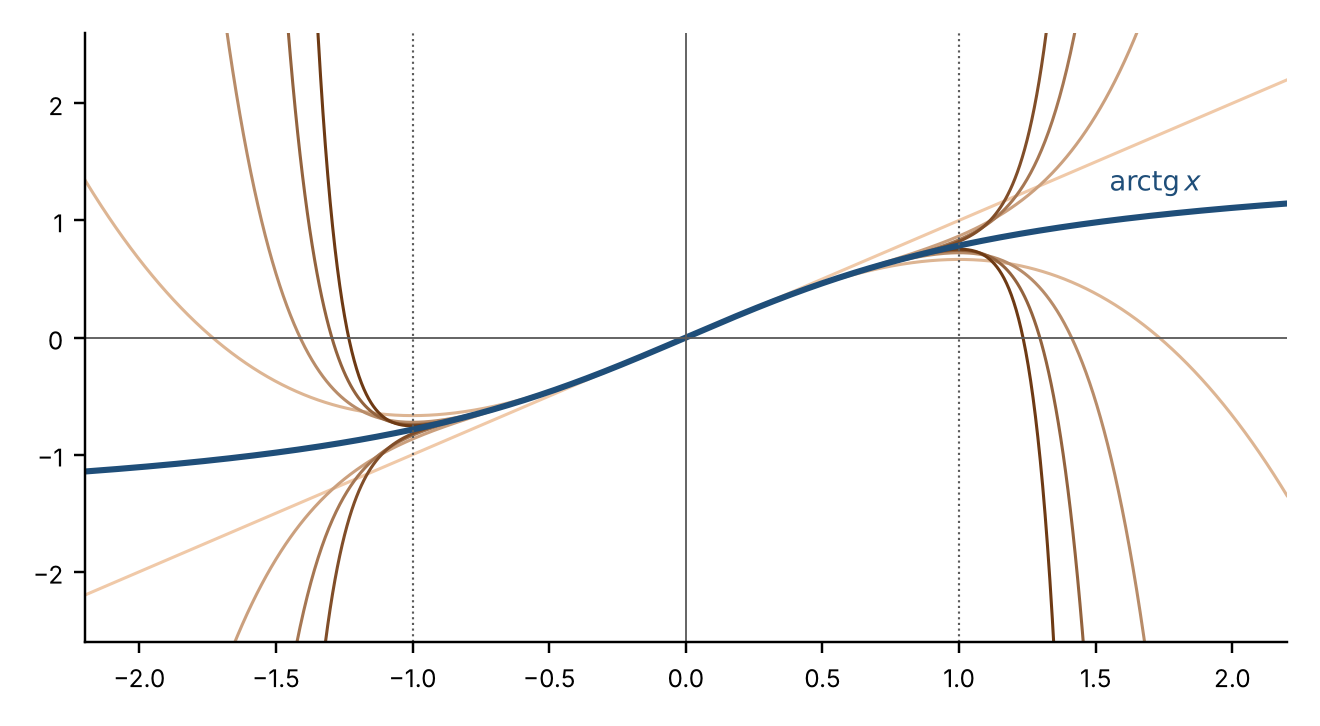
\includegraphics[width=\textwidth]{figure/taylor_arctg.png}
\caption{L'arcotangente (blu) e i suoi polinomi di Taylor in $0$ di grado $1,3,5,\dots,15$
(rame, più scuri al crescere del grado). In $[-1,1]$ i polinomi si avvicinano alla
funzione; per $\abs x>1$ se ne allontanano sempre di più
(\texttt{python/fig\_taylor\_arctg.py}).}
\label{fig:taylor-arctg}
\end{figure}

\begin{python}[Le cifre di $\pi$: serie di Leibniz e formula di Machin]
from fractions import Fraction as F
import math

def arctg(x, n):
    """T(x) = x - x^3/3 + ... + (-1)^n x^(2n+1)/(2n+1)."""
    return sum((-1)**k * x**(2*k + 1) / (2*k + 1)
               for k in range(n + 1))

for n in (10, 100, 1000):
    print(f"Leibniz, n = {n:4d}:  4*T = {4 * arctg(1.0, n):.10f}")
for n in (2, 4, 6, 8):
    p = 4 * (4 * arctg(F(1, 5), n) - arctg(F(1, 239), n))
    print(f"Machin,  n = {n}:     4*T = {float(p):.15f}")
print(f"                  pi    = {math.pi:.15f}")
\end{python}
\begin{risultato}
Leibniz, n =   10:  4*T = 3.2323158094
Leibniz, n =  100:  4*T = 3.1514934011
Leibniz, n = 1000:  4*T = 3.1425916543
Machin,  n = 2:     4*T = 3.141621029325035
Machin,  n = 4:     4*T = 3.141592682404399
Machin,  n = 6:     4*T = 3.141592653623555
Machin,  n = 8:     4*T = 3.141592653589836
                  pi    = 3.141592653589793
\end{risultato}

\begin{idea}[La distanza dell'orizzonte]
Da un velivolo che vola alla quota $h$ sopra una Terra sferica di raggio
$R\approx6371$~km, la visuale verso l'orizzonte è tangente alla superficie
(\cref{fig:orizzonte}). Se $\vartheta$ è l'angolo al centro della Terra tra la verticale del
velivolo e il punto di tangenza, il triangolo rettangolo formato dal centro, dal velivolo
e dal punto di tangenza dà $\cos\vartheta=\frac R{R+h}$, cioè $1-\cos\vartheta=\frac h{R+h}$, e la
distanza dell'orizzonte misurata sulla superficie è $d=R\vartheta$. Per la
\eqref{eq:taylor-cos}, $1-\cos\vartheta=\frac{\vartheta^{2}}2\,(1+o(1))$ per $\vartheta\to0$; poiché $h$ è piccolo
rispetto a $R$, anche $\vartheta$ è piccolo, e
\begin{equation}\label{eq:orizzonte}
  \vartheta\approx\sqrt{\frac{2h}{R}}, \qquad d\approx\sqrt{2Rh} .
\end{equation}
A $10\,000$~m di quota l'orizzonte dista circa $\sqrt{2\cdot6371\cdot10}\approx357$~km. La stessa
formula dà la portata «ottica» di un radar o di un collegamento radio in visibilità; in
radiotecnica, per tener conto della rifrazione atmosferica, si usa un raggio terrestre
equivalente pari ai $\frac43$ di quello reale. Il programma confronta la formula
approssimata con quella esatta $d=R\arccos\frac R{R+h}$. Si vedrà che l'approssimazione
sovrastima leggermente la distanza; l'\cref{es:orizzonte-secondo-ordine} ne spiega il
motivo e ne calcola l'errore.
\end{idea}

\begin{figure}[htb]
\centering
\begin{tikzpicture}[scale=1.0]
  \fill[blu!8] (0,0) circle (2.2);
  \draw[blu, thick] (0,0) circle (2.2);
  \coordinate (O) at (0,0);
  \coordinate (A) at (0,3.3);
  \coordinate (T) at ({2.2*sin(48.19)},{2.2*cos(48.19)});
  \draw[grigio] (O) -- (A);
  \draw[grigio] (O) -- (T);
  \draw[rame, thick] (A) -- (T) -- ($(T)!-0.35!(A)$);
  \fill[rame] (A) circle (1.8pt) node[above, font=\scriptsize] {velivolo};
  \fill (T) circle (1.4pt) node[above right, font=\scriptsize] {orizzonte};
  \draw[grigio] (0,0.5) arc (90:41.81:0.5);
  \node[font=\scriptsize] at (0.33,0.78) {$\vartheta$};
  \draw[verde!70!black, very thick] (0,2.2) arc (90:41.81:2.2);
  \node[font=\scriptsize, verde!70!black] at (0.8,1.78) {$d$};
  \node[font=\scriptsize, left] at (0,1.1) {$R$};
  \node[font=\scriptsize, left] at (0,2.75) {$h$};
  \coordinate (P) at ($(T)!0.2cm!(O)$);
  \coordinate (Q) at ($(T)!0.2cm!(A)$);
  \draw[grigio] (P) -- ($(P)+(Q)-(T)$) -- (Q);
\end{tikzpicture}
\caption{La distanza dell'orizzonte. La visuale dal velivolo al punto di tangenza è
perpendicolare al raggio; l'angolo al centro $\vartheta$ verifica $\cos\vartheta=\frac R{R+h}$, e
la distanza sulla superficie è l'arco $d=R\vartheta$. La quota è fortemente esagerata.}
\label{fig:orizzonte}
\end{figure}

\begin{python}[Distanza dell'orizzonte: formula esatta e approssimata]
import math

R = 6371.0                                 # raggio terrestre [km]
print(" h [km]   esatta [km]   sqrt(2Rh) [km]   differenza")
for h in (0.1, 1.0, 3.0, 10.0, 12.0):
    d = R * math.acos(R / (R + h))         # arco R*theta
    a = math.sqrt(2 * R * h)
    print(f"{h:6.1f}   {d:10.2f}    {a:12.2f}     {a - d:8.3f}")
\end{python}
\begin{risultato}
 h [km]   esatta [km]   sqrt(2Rh) [km]   differenza
   0.1        35.70           35.70        0.000
   1.0       112.87          112.88        0.007
   3.0       195.48          195.51        0.038
  10.0       356.73          356.96        0.233
  12.0       390.72          391.03        0.307
\end{risultato}

\begin{notastorica}[Madhava, Gregory, Leibniz, Machin]
Lo sviluppo dell'arcotangente fu scoperto in India, intorno al 1400, da Madhava di
Sangamagrama, fondatore della scuola astronomica e matematica del Kerala, che ne ricavò
anche la serie \eqref{eq:serie-leibniz}; i suoi risultati, tramandati in testi in sanscrito
e in malayalam, rimasero sconosciuti in Europa. Qui la serie fu riscoperta da James Gregory
(1671) e da Leibniz (1673--1674), che vi giunse con il suo teorema di trasmutazione. Nel
1706 l'astronomo inglese John Machin, con la formula \eqref{eq:machin}, calcolò cento
cifre decimali di $\pi$ a mano; formule dello stesso tipo sono state usate nei record di
calcolo di $\pi$ fino al 2002, quando Yasumasa Kanada ne calcolò con il computer più di
mille miliardi di cifre.
\end{notastorica}

%% ----------------------------------------------------------------------------
%%  §10.2  L'algebra degli o piccoli e il calcolo dei limiti
%% ----------------------------------------------------------------------------
\section{L'algebra degli o piccoli e il calcolo dei limiti}
\label{sec:o-piccoli}

La formula di Taylor con il resto di Peano è lo strumento più efficace per il calcolo
dei limiti che si presentano in forma indeterminata. Cominciamo con un esempio, che ci
mostrerà di quali regole di calcolo abbiamo bisogno.

\begin{esempio}\label{es:limite-taylor-1}
Calcoliamo
\begin{equation}\label{eq:limite-taylor-1}
  \lim_{x\to0}\Bigl(\frac1{x^{2}}-\frac1{x\sen x}\Bigr) ,
\end{equation}
che si presenta nella forma indeterminata $+\infty-(+\infty)$. Riducendo allo stesso
denominatore e usando lo sviluppo $\sen x=x-\frac{x^{3}}6+o(x^{4})$ (la \eqref{eq:taylor-sen} con
$n=1$),
\[
  \frac1{x^{2}}-\frac1{x\sen x}=\frac{\sen x-x}{x^{2}\sen x}
  =\frac{-\frac{x^{3}}6+o(x^{4})}{x^{3}-\frac{x^{5}}6+o(x^{6})} ,
\]
dove abbiamo usato il fatto che $x^{2}\cdot o(x^{4})=o(x^{6})$. Dividendo numeratore e
denominatore per $x^{3}$, e osservando che $\frac{o(x^{4})}{x^{3}}=x\cdot\frac{o(x^{4})}{x^{4}}\to0$ e che
$\frac{o(x^{6})}{x^{3}}\to0$, si ottiene
\[
  \lim_{x\to0}\frac{-\frac16+\frac{o(x^{4})}{x^{3}}}{1-\frac{x^{2}}6+\frac{o(x^{6})}{x^{3}}}=-\frac16 .
\]
Si noti la scelta dell'ordine dello sviluppo. Con il solo $\sen x=x+o(x^{2})$ il numeratore
sarebbe stato $o(x^{2})$, e il rapporto $\frac{o(x^{2})}{x^{3}}$ è ancora indeterminato: occorre
spingere lo sviluppo fino al primo termine che \emph{non si elide}.
\end{esempio}

Nel calcolo precedente abbiamo trattato il simbolo $o(\cdot)$ come se fosse un numero,
sommandolo, moltiplicandolo per potenze, dividendolo. Occorre dare un senso preciso a
queste operazioni.

\begin{notazione}[Uguaglianze con gli o piccoli]
In una formula, il simbolo $o(x^{n})$ (per $x\to0$) indica \emph{una qualsiasi} funzione $f$
tale che $\frac{f(x)}{x^{n}}\to0$; per $n=0$, $o(1)$ indica una qualsiasi funzione infinitesima.
Un'uguaglianza tra espressioni che contengono simboli $o$, come $x^{2}\cdot o(x^{4})=o(x^{6})$,
significa: \emph{ogni} funzione della forma scritta a sinistra è anche della forma
scritta a destra. Queste uguaglianze vanno quindi lette da sinistra a destra, e non sono
simmetriche: $o(x^{2})=o(x)$ è vera (ogni funzione che è $o(x^{2})$ è anche $o(x)$), mentre
$o(x)=o(x^{2})$ è falsa (si pensi a $x^{3/2}$, per $x>0$).
\end{notazione}

\begin{proposizione}[Algebra degli o piccoli]\label{prop:algebra-o}
Per $x\to0$ e per ogni coppia di interi $m,n\ge0$ valgono le proprietà
\begin{align}
  & o(x^{n})+o(x^{n})=o(x^{n}), \qquad o(x^{n})-o(x^{n})=o(x^{n}); \label{eq:o-somma}\\
  & c\cdot o(x^{n})=o(x^{n}), \qquad o(c\,x^{n})=o(x^{n}) \qquad (c\neq0 \text{ costante}); \label{eq:o-costante}\\
  & x^{m}\cdot o(x^{n})=o(x^{m+n}); \label{eq:o-potenza}\\
  & o(x^{m})\cdot o(x^{n})=o(x^{m+n}); \label{eq:o-prodotto}\\
  & o(x^{m})=o(x^{n}) \ \text{ se } m\ge n, \qquad x^{m}=o(x^{n}) \ \text{ se } m>n; \label{eq:o-ordine}\\
  & \frac{o(x^{n})}{x^{m}}=o(x^{n-m}) \qquad (m\le n); \label{eq:o-quoziente}\\
  & o\bigl(o(x^{n})\bigr)=o(x^{n}); \label{eq:o-o}\\
  & o\bigl(x^{n}+o(x^{n})\bigr)=o(x^{n}). \label{eq:o-somma-interna}
\end{align}
\end{proposizione}

\begin{schema}
\Ipotesi{$x\to0$; \ $m,n\ge0$ interi; \ ogni simbolo $o(g)$ denota una funzione $f$ con
$\frac fg\to0$.}
\Tesi{ogni funzione della forma a primo membro delle
\eqref{eq:o-somma}--\eqref{eq:o-somma-interna} è anche della forma a secondo membro.}
\end{schema}

\begin{strategia}
Ogni proprietà si traduce in un'affermazione sui limiti: si scrivono esplicitamente le
funzioni che compaiono a primo membro, si divide per la potenza che compare a secondo
membro e si riconosce, con un'opportuna moltiplicazione e divisione, un prodotto o una
somma di quozienti che tendono a zero per ipotesi. Le ultime due proprietà, in cui un o
piccolo compare \emph{dentro} un altro, richiedono di passare attraverso la funzione
intermedia.
\end{strategia}

\begin{dimostrazione}
Siano $f$ e $g$ funzioni definite vicino a $0$ (escluso al più $0$).

\eqref{eq:o-somma}: se $\frac{f(x)}{x^{n}}\to0$ e $\frac{g(x)}{x^{n}}\to0$, allora
$\frac{f(x)\pm g(x)}{x^{n}}=\frac{f(x)}{x^{n}}\pm\frac{g(x)}{x^{n}}\to0$.

\eqref{eq:o-costante}: se $\frac{f(x)}{x^{n}}\to0$ allora $\frac{c\,f(x)}{x^{n}}=c\,\frac{f(x)}{x^{n}}\to0$; se invece
$\frac{f(x)}{c\,x^{n}}\to0$, allora $\frac{f(x)}{x^{n}}=c\,\frac{f(x)}{c\,x^{n}}\to0$.

\eqref{eq:o-potenza}: se $\frac{f(x)}{x^{n}}\to0$, allora $\frac{x^{m}f(x)}{x^{m+n}}=\frac{f(x)}{x^{n}}\to0$.

\eqref{eq:o-prodotto}: se $\frac{f(x)}{x^{m}}\to0$ e $\frac{g(x)}{x^{n}}\to0$, allora
$\frac{f(x)g(x)}{x^{m+n}}=\frac{f(x)}{x^{m}}\cdot\frac{g(x)}{x^{n}}\to0$.

\eqref{eq:o-ordine}: se $m\ge n$ e $\frac{f(x)}{x^{m}}\to0$, allora $\frac{f(x)}{x^{n}}=x^{m-n}\,\frac{f(x)}{x^{m}}\to0$,
perché $x^{m-n}$ vale $1$ se $m=n$ e tende a $0$ se $m>n$. Se $m>n$, inoltre,
$\frac{x^{m}}{x^{n}}=x^{m-n}\to0$.

\eqref{eq:o-quoziente}: se $\frac{f(x)}{x^{n}}\to0$, allora $\frac{f(x)/x^{m}}{x^{n-m}}=\frac{f(x)}{x^{n}}\to0$.

\eqref{eq:o-o}: sia $g=o(x^{n})$, con $g(x)\neq0$ per $x\neq0$ (condizione richiesta dalla
\cref{def:o-piccolo} perché abbia senso scrivere $o(g)$), e sia $f=o(g)$. Allora
\[
  \frac{f(x)}{x^{n}}=\frac{f(x)}{g(x)}\cdot\frac{g(x)}{x^{n}}\longrightarrow0\cdot0=0 .
\]

\eqref{eq:o-somma-interna}: sia $g(x)=x^{n}+h(x)$ con $h=o(x^{n})$, e sia $f=o(g)$. Poiché
$\frac{g(x)}{x^{n}}=1+\frac{h(x)}{x^{n}}\to1$, la funzione $g$ è diversa da zero vicino a $0$ (per la
permanenza del segno), e
\[
  \frac{f(x)}{x^{n}}=\frac{f(x)}{g(x)}\cdot\frac{g(x)}{x^{n}}
  =\frac{f(x)}{g(x)}\cdot\Bigl(1+\frac{h(x)}{x^{n}}\Bigr)\longrightarrow0\cdot1=0 . \qedhere
\]
\end{dimostrazione}

\begin{attenzione}
Non è lecito scrivere $o(x^{n})-o(x^{n})=0$: i due simboli denotano, in generale, due funzioni
\emph{diverse}, entrambe trascurabili rispetto a $x^{n}$, e la loro differenza è soltanto
un'altra funzione trascurabile rispetto a $x^{n}$, come afferma la \eqref{eq:o-somma}. Ad
esempio $x^{3}=o(x^{2})$ e $2x^{3}=o(x^{2})$, ma $x^{3}-2x^{3}=-x^{3}\neq0$. Per la stessa ragione un
rapporto come $\frac{o(x^{n})}{o(x^{n})}$ non ha alcun significato preciso: può tendere a qualunque
valore, o non avere limite.
\end{attenzione}

Le proprietà \eqref{eq:o-o} e \eqref{eq:o-somma-interna} si generalizzano a un argomento che
sia un qualunque infinitesimo con parte principale nota; è la forma che useremo più
spesso.

\begin{corollario}[o piccoli di infinitesimi con parte principale]\label{cor:o-composto}
Sia $\varphi(x)=a\,x^{k}+o(x^{k})$ per $x\to0$, con $a\neq0$ e $k\ge1$. Allora, per ogni intero
$m\ge1$,
\begin{equation}\label{eq:o-composto}
  \varphi(x)^{m}=a^{m}x^{km}+o(x^{km}), \qquad o\bigl(\varphi(x)^{m}\bigr)=o(x^{km}) .
\end{equation}
\end{corollario}

\begin{schema}
\Ipotesi{$\frac{\varphi(x)}{x^{k}}\to a\neq0$ per $x\to0$; \ $m\ge1$ intero.}
\Tesi{$\frac{\varphi(x)^{m}}{x^{km}}\to a^{m}$; \ se $\frac{f(x)}{\varphi(x)^{m}}\to0$, allora $\frac{f(x)}{x^{km}}\to0$.}
\end{schema}

\begin{strategia}
Tutto discende dal fatto che il rapporto $\frac{\varphi(x)}{x^{k}}$ tende ad $a\neq0$: la potenza
$m$-esima di questo rapporto tende ad $a^{m}$, il che dà la prima uguaglianza. Per la
seconda si procede come per la \eqref{eq:o-o}, scrivendo $\frac{f}{x^{km}}$ come prodotto di
$\frac{f}{\varphi^{m}}$, che tende a zero, e di $\bigl(\frac{\varphi}{x^{k}}\bigr)^{m}$, che resta limitato;
la permanenza del segno garantisce che $\varphi$ non si annulli vicino a $0$.
\end{strategia}

\begin{dimostrazione}
Per ipotesi $\frac{\varphi(x)}{x^{k}}=a+\frac{o(x^{k})}{x^{k}}\to a$, e quindi
$\frac{\varphi(x)^{m}}{x^{km}}=\bigl(\frac{\varphi(x)}{x^{k}}\bigr)^{m}\to a^{m}$, cioè
$\varphi(x)^{m}-a^{m}x^{km}=o(x^{km})$. In particolare $\varphi(x)\neq0$ vicino a $0$, per la permanenza
del segno. Se poi $f=o(\varphi^{m})$,
\[
  \frac{f(x)}{x^{km}}=\frac{f(x)}{\varphi(x)^{m}}\cdot\Bigl(\frac{\varphi(x)}{x^{k}}\Bigr)^{m}\longrightarrow0\cdot a^{m}=0 .
  \qedhere
\]
\end{dimostrazione}

Con questo corollario sono giustificati i calcoli fatti nel \cref{sec:taylor-peano} per la
funzione $1+\sen(e^{x}-1)$: con $u=e^{x}-1=x+o(x)$, si ha $u^{3}=x^{3}+o(x^{3})$ e
$o(u^{3})=o(x^{3})$.

Gli sviluppi di Taylor permettono di confrontare tra loro gli infinitesimi in modo
preciso. Fissiamo il linguaggio.

\begin{definizione}[Ordine di infinitesimo, parte principale, equivalenza]
\label{def:parte-principale}\index{infinitesimo!ordine di}\index{parte principale}
Sia $f$ definita vicino a $0$ (escluso al più $0$). Se esistono un numero $a\neq0$ e un
intero $p\ge0$ tali che
\[
  f(x)=a\,x^{p}+o(x^{p}) \qquad (x\to0),
\]
cioè $\frac{f(x)}{x^{p}}\to a\neq0$, si dice che $f$ è un \emph{infinitesimo di ordine $p$} (se $p\ge1$)
e che $a\,x^{p}$ è la sua \emph{parte principale}. Due funzioni $f$ e $g$ si dicono
\emph{equivalenti} per $x\to0$, e si scrive $f\sim g$, se $\frac{f(x)}{g(x)}\to1$.
\end{definizione}

Ad esempio $\sen x-x$ è un infinitesimo di ordine $3$ con parte principale $-\frac{x^{3}}6$, e
$1-\cos x\sim\frac{x^{2}}2$. Il numero $a$ e l'esponente $p$, quando esistono, sono univocamente
determinati: se fosse anche $f(x)=b\,x^{q}+o(x^{q})$ con $q\neq p$, ad esempio $q>p$ (l'altro
caso è simmetrico), dividendo per $x^{p}$ si avrebbe $\frac{f(x)}{x^{p}}\to0\neq a$; e se $q=p$,
allora $a=b=\lim\frac{f(x)}{x^{p}}$. Una funzione con una parte
principale è equivalente a essa. La proposizione che segue riassume il metodo con cui la
formula di Taylor si usa nel calcolo dei limiti di rapporti.

\begin{proposizione}[Principio della parte principale]\label{prop:parte-principale}
Siano $f(x)=a\,x^{p}+o(x^{p})$ e $g(x)=b\,x^{q}+o(x^{q})$ per $x\to0$, con $a,b\neq0$ e
$p,q\ge0$ interi. Allora
\begin{equation}\label{eq:parte-principale}
  \frac{f(x)}{g(x)}=\frac ab\,x^{p-q}\bigl(1+o(1)\bigr) ;
\end{equation}
in particolare $\frac{f(x)}{g(x)}\to\frac ab$ se $p=q$, e $\frac{f(x)}{g(x)}\to0$ se $p>q$, mentre se $p<q$ il
rapporto diverge in valore assoluto.
\end{proposizione}

\begin{schema}
\Ipotesi{$\frac{f(x)}{x^{p}}\to a\neq0$, \ $\frac{g(x)}{x^{q}}\to b\neq0$ per $x\to0$.}
\Tesi{$\frac{f(x)}{g(x)}\sim\frac ab\,x^{p-q}$: nel limite di un rapporto si possono sostituire numeratore
e denominatore con le loro parti principali.}
\end{schema}

\begin{strategia}
Si confronta il rapporto $\frac fg$ con il rapporto delle parti principali, cioè si mostra
che il loro quoziente tende a $1$. Dividendo numeratore per $x^{p}$ e denominatore per
$x^{q}$, questo quoziente diventa il prodotto di $\frac{f(x)/x^{p}}{a}$ e di
$\frac{b}{g(x)/x^{q}}$, che tendono entrambi a $1$ per ipotesi. Il comportamento di $x^{p-q}$
decide poi il limite.
\end{strategia}

\begin{dimostrazione}
Per $x\neq0$ vicino a $0$ (dove $g(x)\neq0$, per la permanenza del segno applicata a
$\frac{g(x)}{x^{q}}\to b\neq0$),
\[
  \frac{f(x)}{g(x)}\cdot\frac b{a\,x^{p-q}}=\frac{f(x)/x^{p}}{a}\cdot\frac{b}{g(x)/x^{q}}\longrightarrow\frac aa\cdot\frac bb=1 .
\]
Le affermazioni sul limite seguono perché $x^{p-q}$ vale $1$ se $p=q$, tende a $0$ se $p>q$
e diverge in valore assoluto se $p<q$.
\end{dimostrazione}

Nell'\cref{es:limite-taylor-1}, ad esempio, il numeratore $\sen x-x$ ha parte principale
$-\frac{x^{3}}6$ e il denominatore $x^{2}\sen x$ ha parte principale $x^{3}$: il limite è $-\frac16$, senza
altri calcoli. Il problema si riduce dunque a trovare la parte principale del numeratore
e del denominatore, cioè il primo termine non nullo dei loro sviluppi.

\begin{esempio}\label{es:limite-taylor-2}
Calcoliamo
\[
  \lim_{x\to0}\Bigl(\frac1x-\frac{\cos x}{x^{3}}+\frac{\sen3x}{3x^{4}}\Bigr)
  =\lim_{x\to0}\frac{3x^{3}-3x\cos x+\sen3x}{3x^{4}} .
\]
Il denominatore ha parte principale $3x^{4}$; occorre dunque sviluppare il numeratore
almeno fino all'ordine $4$. Ponendo $3x$ al posto di $x$ nello sviluppo del seno
(\cref{lem:sostituzione-o} e \eqref{eq:o-costante}) si ottiene $\sen3x=3x-\frac92\,x^{3}+o(x^{4})$;
inoltre, per la \eqref{eq:taylor-cos} e la \eqref{eq:o-potenza},
$3x\cos x=3x\bigl(1-\frac{x^{2}}2+o(x^{3})\bigr)=3x-\frac32\,x^{3}+o(x^{4})$. Allora
\[
  3x^{3}-3x\cos x+\sen3x=3x^{3}-3x+\frac32\,x^{3}+3x-\frac92\,x^{3}+o(x^{4})=o(x^{4}) ,
\]
e il limite vale $\lim_{x\to0}\frac{o(x^{4})}{3x^{4}}=0$. Tutti i termini fino all'ordine $4$ si sono
elisi. Spingendo gli sviluppi di un ordine (o di due) si trova la parte principale del
numeratore, $\frac{19}{10}\,x^{5}$, e quindi, per la \cref{prop:parte-principale}, la funzione
tende a zero come $\frac{19}{30}\,x$ (\cref{es:verifica-19-30}).
\end{esempio}

\begin{esempio}\label{es:limite-taylor-3}
Studiamo il limite della successione
\[
  \lim_{n\to+\infty}\Bigl(\cos\frac1n\Bigr)^{-n^{2}} .
\]
Per la definizione di limite di funzione mediante successioni (\cref{def:limite-funzione}),
con $x_{n}=\frac1n\to0$, basta calcolare il limite di funzione
\[
  \lim_{x\to0}(\cos x)^{-1/x^{2}}=\lim_{x\to0}e^{-\frac{\log\cos x}{x^{2}}} ,
\]
che è della forma indeterminata $1^{\infty}$. Dalla \eqref{eq:taylor-cos}, $\cos x=1+u$ con
$u=-\frac{x^{2}}2+o(x^{3})$; dalla \eqref{eq:taylor-log} con $n=1$, $\log(1+u)=u+o(u)$, e per il
\cref{cor:o-composto} (con $a=-\frac12$, $k=2$, $m=1$) $o(u)=o(x^{2})$. Dunque
\[
  \log\cos x=-\frac{x^{2}}2+o(x^{3})+o(x^{2})=-\frac{x^{2}}2+o(x^{2}) ,
\]
e quindi $-\frac{\log\cos x}{x^{2}}\to\frac12$. Per la continuità dell'esponenziale (\cref{teo:continuita-esponenziale}) entrambi i
limiti valgono $e^{1/2}=\sqrt e$.
\end{esempio}

\begin{figure}[htb]
\centering
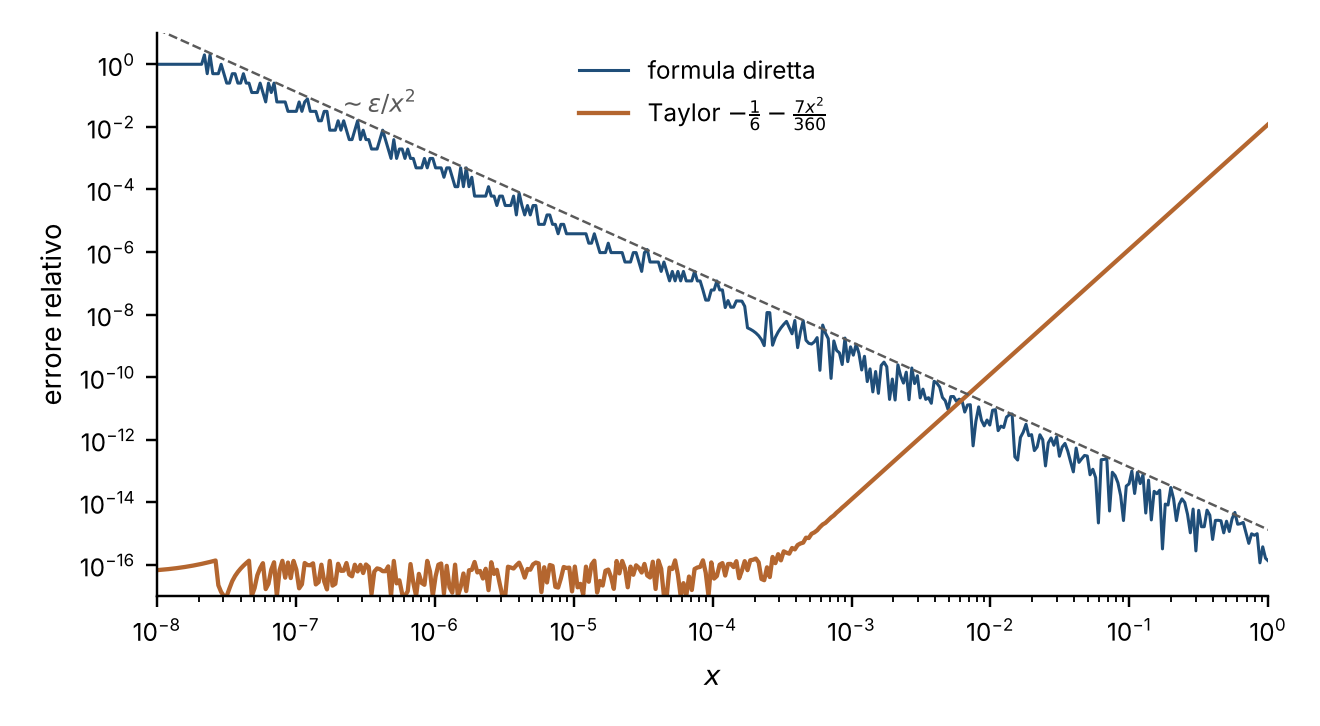
\includegraphics[width=\textwidth]{figure/cancellazione.png}
\caption{Errore relativo nel calcolo di $f(x)=\frac1{x^{2}}-\frac1{x\sen x}$ in aritmetica a
virgola mobile (precisione doppia). La formula diretta (blu) perde cifre come
$\frac{\varepsilon}{x^{2}}$, con $\varepsilon\approx2{,}2\cdot10^{-16}$, per la cancellazione tra due numeri quasi
uguali; il polinomio di Taylor $-\frac16-\frac{7x^{2}}{360}$ (rame) ha un errore che decresce come
$x^{4}$. Le due curve si incrociano per $x$ dell'ordine di $10^{-2}$
(\texttt{python/fig\_cancellazione.py}).}
\label{fig:cancellazione}
\end{figure}

La formula di Taylor non serve soltanto a calcolare limiti «a mano»: è indispensabile
anche nel calcolo numerico. Nel \cref{cap:funzioni-continue} abbiamo incontrato il
fenomeno della \emph{cancellazione}, a proposito di $1-\cos x$ e delle funzioni
\texttt{log1p} ed \texttt{expm1}. La funzione dell'\cref{es:limite-taylor-1}, calcolata con
un computer per $x$ piccolo, ne è un esempio estremo: è la differenza di due numeri
grandi e quasi uguali, ciascuno affetto da un errore di arrotondamento relativo
dell'ordine di $\varepsilon\approx2{,}2\cdot10^{-16}$, e quindi da un errore assoluto dell'ordine di
$\frac\varepsilon{x^{2}}$, che la sottrazione non elimina. Per $x=10^{-8}$ il risultato è privo di
significato. Lo sviluppo $-\frac16-\frac{7x^{2}}{360}+o(x^{3})$ non soffre di questo difetto
(\cref{fig:cancellazione}): la formula di Taylor è il rimedio \emph{sistematico} alla
cancellazione, perché esegue la sottrazione «sulla carta», una volta per tutte. Le
librerie numeriche seguono la stessa idea: per $x$ vicino a zero calcolano funzioni come
\texttt{expm1} e \texttt{log1p} con approssimazioni polinomiali o razionali costruite in
modo da non formare la differenza (i loro coefficienti non sono esattamente quelli di
Taylor, come vedremo nel \cref{sec:tabulazione}), e passano alla formula diretta soltanto
quando la cancellazione non è più pericolosa.

\begin{python}[Limiti con la formula di Taylor: verifica simbolica e numerica]
import math
import sympy as sp
from mpmath import mp, mpf, sin as msin

x = sp.symbols('x')
f = 1 / x**2 - 1 / (x * sp.sin(x))
print(sp.series(f, x, 0, 4))
g = 1 / x - sp.cos(x) / x**3 + sp.sin(3 * x) / (3 * x**4)
print(sp.series(g, x, 0, 3))
print(sp.limit(sp.cos(x)**(-1 / x**2), x, 0))

mp.dps = 40                         # 40 cifre: valore "esatto"
print("     x      formula diretta      Taylor       esatto")
for k in (1, 3, 5, 7, 8):
    t = 10.0**(-k)
    d = 1 / t**2 - 1 / (t * math.sin(t))
    p = -1 / 6 - 7 * t**2 / 360
    e = 1 / mpf(t)**2 - 1 / (mpf(t) * msin(mpf(t)))
    print(f"  1e-{k}  {d:17.12f}  {p:14.12f}  {float(e):14.12f}")
\end{python}
\begin{risultato}
-1/6 - 7*x**2/360 + O(x**4)
19*x/30 + O(x**3)
exp(1/2)
     x      formula diretta      Taylor       esatto
  1e-1    -0.166861316348  -0.166861111111  -0.166861316348
  1e-3    -0.166666686186  -0.166666686111  -0.166666686111
  1e-5    -0.166667938232  -0.166666666669  -0.166666666669
  1e-7    -0.156250000000  -0.166666666667  -0.166666666667
  1e-8     0.000000000000  -0.166666666667  -0.166666666667
\end{risultato}

\begin{notastorica}[I simboli di Landau]
Il simbolo $O$ («o grande»: $f=O(g)$ se $\frac fg$ è limitato) fu introdotto dal teorico dei
numeri tedesco Paul Bachmann nel 1894, nel secondo volume della sua \emph{Zahlentheorie}.
Edmund Landau lo adottò e vi affiancò il simbolo $o$ nel suo trattato sulla distribuzione
dei numeri primi (1909), e da allora entrambi portano il suo nome. L'uso sistematico
degli sviluppi di Taylor per il calcolo dei limiti, però, è molto più antico: già i
matematici del Settecento, a partire da Eulero, trattavano le funzioni come «polinomi
infiniti» e ne confrontavano i termini di grado più basso, anche se senza un controllo
rigoroso del resto. È proprio questo controllo che i simboli di Landau e la formula di
Peano permettono di esercitare con poca fatica.
\end{notastorica}

%% ----------------------------------------------------------------------------
%%  §10.3  La formula di Taylor con il resto integrale
%% ----------------------------------------------------------------------------
\section{La formula di Taylor con il resto integrale}
\label{sec:resto-integrale}

Il resto di Peano descrive il comportamento dell'errore $R_{n}(x)=f(x)-T_{n}(x)$ per
$x\to x_{0}$, ma non dice nulla sul suo valore per un $x$ \emph{fissato}: sapere che
$R_{n}(x)=o\bigl((x-x_{0})^{n}\bigr)$ non permette di affermare, ad esempio, che l'errore
commesso calcolando $\sen\frac1{10}$ con il polinomio $x-\frac{x^{3}}6$ è minore di $10^{-7}$. Per
questo occorre un'espressione esplicita del resto. Se la funzione è abbastanza regolare,
il calcolo integrale la fornisce.

\begin{teorema}[Formula di Taylor con il resto integrale]\label{teo:resto-integrale}
\index{formula di Taylor!con il resto integrale}
Sia $f$ derivabile $n+1$ volte nell'intervallo $[a,b]$, con derivata $f^{(n+1)}$ continua
(cioè $f$ di classe $C^{n+1}$ in $[a,b]$), e sia $x_{0}\in[a,b]$. Allora il resto
$R_{n}(x)=f(x)-T_{n}(x)$ della formula di Taylor di ordine $n$ con centro $x_{0}$ si
rappresenta nella forma
\begin{equation}\label{eq:resto-integrale}
  R_{n}(x)=\int_{x_{0}}^{x}\frac{(x-t)^{n}}{n!}\,f^{(n+1)}(t)\,dt \qquad\perogni x\in[a,b] .
\end{equation}
\end{teorema}

\begin{schema}
\Ipotesi{$f\in C^{n+1}([a,b])$; \ $x_{0}\in[a,b]$.}
\Tesi{$f(x)=\displaystyle\sum_{k=0}^{n}\frac{f^{(k)}(x_{0})}{k!}(x-x_{0})^{k}
+\int_{x_{0}}^{x}\frac{(x-t)^{n}}{n!}\,f^{(n+1)}(t)\,dt$ per ogni $x\in[a,b]$.}
\end{schema}

\begin{strategia}
Procediamo per induzione su $n$. Per $n=0$ la tesi è la formula fondamentale del calcolo
integrale: $f(x)-f(x_{0})=\int_{x_{0}}^{x}f'(t)\,dt$. Per passare da $n$ a $n+1$ osserviamo che
$R_{n}$ e $R_{n+1}$ differiscono per un solo termine,
$R_{n}(x)-R_{n+1}(x)=\frac{f^{(n+1)}(x_{0})}{(n+1)!}(x-x_{0})^{n+1}$: dobbiamo «estrarre» questo termine
dall'integrale \eqref{eq:resto-integrale}. Lo strumento è l'integrazione per parti nella
variabile $t$ (con $x$ fissato), derivando $f^{(n+1)}$ e integrando il peso
$\frac{(x-t)^{n}}{n!}$, la cui primitiva $-\frac{(x-t)^{n+1}}{(n+1)!}$ si annulla per $t=x$: in questo modo il
termine di bordo in $t=x$ scompare, e quello in $t=x_{0}$ è proprio il termine cercato.
\end{strategia}

\begin{dimostrazione}
Dimostriamo per induzione su $n\ge0$ la proposizione
\begin{quote}
$P(n)$: \emph{per ogni funzione $f$ di classe $C^{n+1}$ in $[a,b]$ e per ogni
$x_{0},x\in[a,b]$ vale la \eqref{eq:resto-integrale}.}
\end{quote}

\emph{Base} ($n=0$). Il polinomio di Taylor di ordine $0$ è la costante $f(x_{0})$, e
$R_{0}(x)=f(x)-f(x_{0})$. Poiché $f'$ è continua, per la formula fondamentale del calcolo
integrale (\cref{teo:formula-fondamentale})
\[
  \int_{x_{0}}^{x}f'(t)\,dt=\Bigl[f(t)\Bigr]_{t=x_{0}}^{t=x}=f(x)-f(x_{0})=R_{0}(x) ,
\]
che è la \eqref{eq:resto-integrale} per $n=0$ (si ricordi che $0!=1$ e $(x-t)^{0}=1$).

\emph{Passo induttivo.} Supponiamo vera $P(n)$ e sia $f$ di classe $C^{n+2}$ in $[a,b]$. In
particolare $f$ è di classe $C^{n+1}$, e per l'ipotesi induttiva
\[
  R_{n}(x)=\int_{x_{0}}^{x}\frac{(x-t)^{n}}{n!}\,f^{(n+1)}(t)\,dt .
\]
Fissato $x$, integriamo per parti (\cref{teo:per-parti-definito}) con
$F(t)=f^{(n+1)}(t)$, di classe $C^{1}$, e $G(t)=-\frac{(x-t)^{n+1}}{(n+1)!}$, che ha derivata
$G'(t)=\frac{(x-t)^{n}}{n!}$. Il teorema è enunciato per un intervallo $[\alpha,\beta]$ con $\alpha<\beta$, ma
vale anche quando l'estremo inferiore supera quello superiore, perché scambiando gli
estremi entrambi i membri cambiano segno; possiamo quindi usarlo anche se $x<x_{0}$.
Poiché $G(x)=0$,
\begin{align*}
  R_{n}(x)&=\int_{x_{0}}^{x}G'(t)F(t)\,dt
  =\Bigl[G(t)F(t)\Bigr]_{t=x_{0}}^{t=x}-\int_{x_{0}}^{x}G(t)F'(t)\,dt\\
  &=\frac{(x-x_{0})^{n+1}}{(n+1)!}\,f^{(n+1)}(x_{0})
  +\int_{x_{0}}^{x}\frac{(x-t)^{n+1}}{(n+1)!}\,f^{(n+2)}(t)\,dt .
\end{align*}
D'altra parte $T_{n+1}(x)=T_{n}(x)+\frac{f^{(n+1)}(x_{0})}{(n+1)!}(x-x_{0})^{n+1}$, e quindi
\[
\begin{aligned}
  R_{n+1}(x)&=R_{n}(x)-\frac{f^{(n+1)}(x_{0})}{(n+1)!}(x-x_{0})^{n+1}\\
  &=\int_{x_{0}}^{x}\frac{(x-t)^{n+1}}{(n+1)!}\,f^{(n+2)}(t)\,dt ,
\end{aligned}
\]
che è la \eqref{eq:resto-integrale} con $n+1$ al posto di $n$. Dunque vale $P(n+1)$, e per il
principio di induzione la tesi è dimostrata per ogni $n$.
\end{dimostrazione}

\begin{osservazione}[Il significato del peso]
La \eqref{eq:resto-integrale} dice che l'errore è una «media pesata» della derivata
$f^{(n+1)}$ lungo l'intervallo di estremi $x_{0}$ e $x$, con peso $\frac{(x-t)^{n}}{n!}$. Per $n=1$,
\[
  f(x)=f(x_{0})+f'(x_{0})(x-x_{0})+\int_{x_{0}}^{x}(x-t)\,f''(t)\,dt :
\]
la distanza tra il grafico e la retta tangente in $x_{0}$ dipende soltanto dalla derivata
seconda. Se $f''\ge0$, per $x>x_{0}$ l'integrando è non negativo, e per $x<x_{0}$ si ha
$\int_{x_{0}}^{x}(x-t)f''(t)\,dt=\int_{x}^{x_{0}}(t-x)f''(t)\,dt\ge0$: il grafico di una funzione con
derivata seconda non negativa sta sopra ciascuna delle sue rette tangenti, come sappiamo
dallo studio della convessità (\cref{cap:applicazioni-derivate}). Il peso $(x-t)$ è
massimo vicino a $x_{0}$ e nullo in $t=x$: la curvatura che si trova vicino al centro dello
sviluppo «pesa» di più, perché il suo effetto si accumula lungo tutto il tratto
successivo.
\end{osservazione}

\begin{esempio}[L'esponenziale supera i suoi polinomi di Taylor]\label{es:exp-maggiore-taylor}
Sia $f(x)=e^{x}$, $x_{0}=0$. Poiché $f^{(n+1)}(t)=e^{t}>0$, per $x>0$ l'integrando della
\eqref{eq:resto-integrale} è positivo in $(0,x)$, e quindi $R_{n}(x)>0$:
\begin{equation}\label{eq:exp-maggiore-taylor}
  e^{x}>1+x+\frac{x^{2}}2+\dots+\frac{x^{n}}{n!} \qquad\perogni x>0,\ \perogni n\ge0 .
\end{equation}
In particolare, con $x=1$, $e>\sum_{k=0}^{n}\frac1{k!}$ per ogni $n$: le somme $\sum_{k=0}^{n}\frac1{k!}$ sono
approssimazioni \emph{per difetto} di $e$. Nel \cref{sec:tabulazione} maggioreremo
l'errore $R_{n}(1)$, e otterremo così anche approssimazioni per eccesso.
\end{esempio}

\subsection{Un'applicazione: la freccia di un'ala a sbalzo}

Il resto integrale ha un'interpretazione fisica immediata nella teoria della trave. Nel
\cref{sec:applicazioni-integrali} abbiamo modellato la semiala come una trave incastrata
alla radice $y=0$ e libera all'estremità $y=s$, caricata dalla portanza distribuita
$l(y)$, e ne abbiamo calcolato il momento flettente
$M(y)=\int_{y}^{s}(\eta-y)\,l(\eta)\,d\eta$ \eqref{eq:taglio-momento}. Indichiamo con $v(y)$ lo
spostamento verticale (la \emph{freccia}) della linea d'asse nella stazione $y$. Nella
teoria di Eulero--Bernoulli la curvatura $\frac1\rho$ della linea d'asse deformata è
proporzionale al momento flettente, $\frac1\rho=\frac M{EI}$, dove $E$ è il modulo di
elasticità del materiale e $I$ il momento d'inerzia del second'ordine della sezione
rispetto all'asse neutro; supponiamo per ora $E$ e $I$ costanti. La curvatura del grafico
di $v$ vale $\frac{v''}{(1+v'^{2})^{3/2}}$ e, per piccole rotazioni ($\abs{v'}\ll1$), si riduce a $v''$.
Con $v$ positivo verso l'alto e $M>0$ per una portanza diretta verso l'alto (la
convenzione del \cref{sec:applicazioni-integrali}; molti testi usano la convenzione
opposta e scrivono $v''=-\frac M{EI}$), si ottiene l'equazione della linea elastica
\begin{equation}\label{eq:linea-elastica}
  v''(y)=\frac{M(y)}{EI} .
\end{equation}
L'incastro impone $v(0)=0$ e $v'(0)=0$: alla radice l'ala non si sposta e non ruota.

\begin{proposizione}[Freccia di una trave a sbalzo]\label{prop:freccia}
Sia $l$ continua in $[0,s]$, e sia $v$ di classe $C^{2}$ in $[0,s]$, soluzione della
\eqref{eq:linea-elastica} con $v(0)=v'(0)=0$. Allora
\begin{equation}\label{eq:freccia}
  v(y)=\frac1{EI}\int_{0}^{y}(y-t)\,M(t)\,dt \qquad\perogni y\in[0,s] .
\end{equation}
In particolare, per un carico uniforme $l(y)=l$ la freccia all'estremità vale
$v(s)=\frac{l\,s^{4}}{8EI}$.
\end{proposizione}

\begin{schema}
\Ipotesi{$l$ continua; \ $v\in C^{2}([0,s])$; \ $v''=\frac M{EI}$; \ $v(0)=v'(0)=0$.}
\Tesi{$v(y)=\frac1{EI}\int_{0}^{y}(y-t)M(t)\,dt$; \ con carico uniforme $v(s)=\frac{ls^{4}}{8EI}$.}
\end{schema}

\begin{strategia}
È la formula di Taylor di ordine $1$ con centro nell'incastro e resto integrale: il
polinomio di Taylor $v(0)+v'(0)y$ è nullo per le condizioni di incastro, e resta soltanto
il resto, in cui $v''$ si sostituisce con la \eqref{eq:linea-elastica}. Per il carico
uniforme si calcola $M$ e un integrale di potenze.
\end{strategia}

\begin{dimostrazione}
Per il \cref{teo:resto-integrale} con $n=1$ e $x_{0}=0$,
\[
  v(y)=v(0)+v'(0)\,y+\int_{0}^{y}(y-t)\,v''(t)\,dt=\frac1{EI}\int_{0}^{y}(y-t)\,M(t)\,dt .
\]
Se $l$ è costante, $M(t)=l\int_{t}^{s}(\eta-t)\,d\eta=\frac l2(s-t)^{2}$, e
\[
  v(s)=\frac l{2EI}\int_{0}^{s}(s-t)^{3}\,dt=\frac l{2EI}\Bigl[-\frac{(s-t)^{4}}4\Bigr]_{0}^{s}
  =\frac{l\,s^{4}}{8EI} . \qedhere
\]
\end{dimostrazione}

\begin{figure}[htb]
\centering
\begin{tikzpicture}[x=1.6cm, y=1.6cm]
  \fill[pattern=north east lines, pattern color=grigio] (-0.25,-0.9) rectangle (0,1.3);
  \draw[thick] (0,-0.9) -- (0,1.3);
  \draw[tratteggio] (0,0) -- (4.2,0);
  \draw[blu, very thick, domain=0:4, samples=60]
    plot (\x, {0.9*(\x/4)^2*(6-4*(\x/4)+(\x/4)^2)/3});
  \foreach \y in {0.25,0.75,...,3.75} {
    \pgfmathsetmacro{\v}{0.9*(\y/4)^2*(6-4*(\y/4)+(\y/4)^2)/3}
    \pgfmathsetmacro{\h}{0.6*sqrt(1-(\y/4)^2)}
    \draw[rame, -{Stealth[length=1.6mm]}] (\y,\v-0.06-\h) -- (\y,\v-0.06);
  }
  \node[rame, font=\scriptsize] at (1.0,-0.62) {$l(y)$};
  \draw[grigio, {Stealth[length=1.2mm]}-{Stealth[length=1.2mm]}] (3,0) -- (3,0.601);
  \node[font=\scriptsize] at (3,0.8) {$v(y)$};
  \draw[{Stealth[length=1.6mm]}-{Stealth[length=1.6mm]}] (4.15,0) -- (4.15,0.9)
    node[midway, right, font=\scriptsize] {$v(s)$};
  \draw[-{Stealth[length=1.8mm]}] (0,-1.05) -- (4.4,-1.05) node[right, font=\scriptsize] {$y$};
  \draw (4,-1.0) -- (4,-1.1) node[below, font=\scriptsize] {$s$};
  \draw (3,-1.0) -- (3,-1.1) node[below, font=\scriptsize] {$y$};
  \node[font=\scriptsize, below] at (0,-1.1) {$0$};
\end{tikzpicture}
\caption{La semiala come trave a sbalzo: incastrata alla radice, si inflette verso l'alto
sotto la portanza distribuita $l(y)$. Il polinomio di Taylor della freccia $v$ con
centro nell'incastro è nullo, e la freccia coincide con il resto integrale
\eqref{eq:freccia}. Gli spostamenti sono fortemente esagerati, e la deformata e il
profilo del carico sono soltanto qualitativi.}
\label{fig:linea-elastica}
\end{figure}

La \eqref{eq:freccia} si legge così: il tratto $[t,t+dt]$ della trave, dove il momento vale
$M(t)$, ruota di un angolo $\frac{M(t)}{EI}\,dt$, e questa rotazione, propagata con braccio $y-t$
fino alla stazione $y$, produce lo spostamento $(y-t)\frac{M(t)}{EI}\,dt$. Il peso $(y-t)$ del
resto integrale è proprio questo braccio. Per la semiala del
\cref{es:taglio-ellittico} ($W=10\,000$~N, $b=10$~m) e una rigidezza flessionale
$EI=2\cdot10^{6}$~N\,m$^{2}$ (un valore puramente indicativo), il carico uniforme
$l=\frac Wb=1000$~N/m dà una freccia all'estremità di circa $3{,}9$~cm; con la
distribuzione ellittica, che concentra la portanza verso la radice, la freccia scende a
circa $3{,}0$~cm, cioè si riduce di circa il $23\%$ (il rapporto esatto è calcolato
nell'\cref{es:freccia-ellittica}). Il programma calcola le due frecce integrando
numericamente. Si noti infine che la dimostrazione della \cref{prop:freccia} non usa la
costanza di $EI$: per un'ala reale, rastremata, la rigidezza $EI(t)$ diminuisce verso
l'estremità, e la stessa formula di Taylor dà $v(y)=\int_{0}^{y}(y-t)\frac{M(t)}{EI(t)}\,dt$, purché
$EI$ sia continua e positiva.

\begin{python}[Freccia all'estremità della semiala]
import math
from scipy.integrate import quad

W, b, EI = 10000.0, 10.0, 2.0e6            # N, m, N*m^2
s = b / 2
carichi = {
    "uniforme": lambda y: W / b,
    "ellittico": lambda y: 4 * W / (math.pi * b)
                           * math.sqrt(max(0.0, 1 - (y / s)**2)),
}
v_tip = {}
for nome, l in carichi.items():
    M = lambda t: quad(lambda e: (e - t) * l(e), t, s)[0]
    v_tip[nome] = quad(lambda t: (s - t) * M(t), 0, s)[0] / EI
    print(f"{nome:9s}:  v(s) = {100 * v_tip[nome]:.3f} cm")
print(f"formula l*s^4/(8EI): {100 * (W/b) * s**4 / (8*EI):.3f} cm")
print(f"rapporto ellittico/uniforme = "
      f"{v_tip['ellittico'] / v_tip['uniforme']:.4f}")
\end{python}
\begin{risultato}
uniforme :  v(s) = 3.906 cm
ellittico:  v(s) = 3.022 cm
formula l*s^4/(8EI): 3.906 cm
rapporto ellittico/uniforme = 0.7736
\end{risultato}

%% ----------------------------------------------------------------------------
%%  §10.4  La formula di Taylor con il resto di Lagrange
%% ----------------------------------------------------------------------------
\section{La formula di Taylor con il resto di Lagrange}
\label{sec:resto-lagrange}

Il resto integrale è esatto, ma per stimarlo non occorre calcolare l'integrale: basta
sapere tra quali valori varia $f^{(n+1)}$. Il peso $\frac{(x-t)^{n}}{n!}$, infatti, non cambia segno
nell'intervallo di integrazione, e per una media pesata con peso di segno costante vale
un analogo del teorema della media (\cref{teo:media}).

\begin{lemma}[Teorema della media pesata]\label{lem:media-pesata}
\index{teorema!della media pesata}
Siano $g$ e $w$ continue in $[\alpha,\beta]$, con $w(t)\ge0$ per ogni $t\in[\alpha,\beta]$. Esiste un punto
$\xi\in[\alpha,\beta]$ tale che
\begin{equation}\label{eq:media-pesata}
  \int_{\alpha}^{\beta}g(t)\,w(t)\,dt=g(\xi)\int_{\alpha}^{\beta}w(t)\,dt .
\end{equation}
\end{lemma}

\begin{schema}
\Ipotesi{$g$, $w$ continue in $[\alpha,\beta]$; \ $w\ge0$.}
\Tesi{$\esiste\xi\in[\alpha,\beta]$ : $\int_{\alpha}^{\beta}g\,w=g(\xi)\int_{\alpha}^{\beta}w$.}
\end{schema}

\begin{strategia}
Si stringe $g$ tra il suo minimo $m$ e il suo massimo $M$ e si moltiplica per $w\ge0$, che
conserva le disuguaglianze; integrando si trova che il rapporto
$\frac{\int gw}{\int w}$ è compreso tra $m$ e $M$, e il teorema dei valori intermedi fornisce il
punto $\xi$. Va trattato a parte il caso $\int w=0$, in cui il rapporto non ha senso.
\end{strategia}

\begin{dimostrazione}
Per il teorema di Weierstrass (\cref{teo:weierstrass}) esistono
$m=\min_{[\alpha,\beta]}g$ e $M=\max_{[\alpha,\beta]}g$. Poiché $w\ge0$, da $m\le g(t)\le M$ segue
$m\,w(t)\le g(t)\,w(t)\le M\,w(t)$ per ogni $t$, e per il confronto tra integrali
(\cref{teo:confronto-integrali}), essendo $gw$ continua e quindi integrabile,
\begin{equation}\label{eq:media-pesata-stima}
  m\int_{\alpha}^{\beta}w(t)\,dt\le\int_{\alpha}^{\beta}g(t)\,w(t)\,dt\le M\int_{\alpha}^{\beta}w(t)\,dt .
\end{equation}
Se $\int_{\alpha}^{\beta}w=0$, la \eqref{eq:media-pesata-stima} dà $\int_{\alpha}^{\beta}gw=0$, e la tesi vale con
qualunque $\xi$. Altrimenti $\int_{\alpha}^{\beta}w>0$, e dividendo si ottiene
$m\le\frac{\int_{\alpha}^{\beta}gw}{\int_{\alpha}^{\beta}w}\le M$. Per il secondo teorema dei valori intermedi
(\cref{teo:valori-intermedi-2}) la funzione continua $g$ assume in $[\alpha,\beta]$ tutti i valori
compresi tra $m$ e $M$: esiste dunque $\xi$ con $g(\xi)=\frac{\int gw}{\int w}$, che è la tesi.
\end{dimostrazione}

Con $w\equiv1$ si ritrova il teorema della media. Applichiamo ora il lemma al resto
integrale.

\begin{teorema}[Formula di Taylor con il resto di Lagrange]\label{teo:resto-lagrange}
\index{formula di Taylor!con il resto di Lagrange}
Sia $f$ derivabile $n+1$ volte in $[a,b]$, con derivata $f^{(n+1)}$ continua, e sia
$x_{0}\in[a,b]$. Per ogni $x\in[a,b]$ esiste un punto $x_{1}$ compreso tra $x_{0}$ e $x$ tale che
\begin{equation}\label{eq:resto-lagrange}
  R_{n}(x)=\frac{f^{(n+1)}(x_{1})}{(n+1)!}\,(x-x_{0})^{n+1} ,
\end{equation}
cioè
\[
  f(x)=\sum_{k=0}^{n}\frac{f^{(k)}(x_{0})}{k!}(x-x_{0})^{k}+\frac{f^{(n+1)}(x_{1})}{(n+1)!}(x-x_{0})^{n+1} .
\]
\end{teorema}

\begin{schema}
\Ipotesi{$f\in C^{n+1}([a,b])$; \ $x_{0},x\in[a,b]$.}
\Tesi{$\esiste x_{1}$ tra $x_{0}$ e $x$ : \ $R_{n}(x)=\frac{f^{(n+1)}(x_{1})}{(n+1)!}(x-x_{0})^{n+1}$.}
\end{schema}

\begin{strategia}
Il resto è l'integrale \eqref{eq:resto-integrale} di $f^{(n+1)}$ contro il peso
$\frac{(x-t)^{n}}{n!}$, che ha segno costante tra $x_{0}$ e $x$. Il \cref{lem:media-pesata} porta
fuori dall'integrale $f^{(n+1)}$, calcolata in un punto intermedio, e l'integrale del peso
si calcola esplicitamente. Se $x<x_{0}$ occorre prima riportare l'integrale a un intervallo
orientato e un peso non negativo, controllando i segni.
\end{strategia}

\begin{dimostrazione}
Se $x=x_{0}$ si ha $R_{n}(x_{0})=0$ e la tesi vale con $x_{1}=x_{0}$.

\emph{Caso $x>x_{0}$.} Il peso $w(t)=\frac{(x-t)^{n}}{n!}$ è continuo e non negativo in
$[x_{0},x]$, e
\begin{equation}\label{eq:integrale-peso}
  \int_{x_{0}}^{x}\frac{(x-t)^{n}}{n!}\,dt=\Bigl[-\frac{(x-t)^{n+1}}{(n+1)!}\Bigr]_{t=x_{0}}^{t=x}
  =\frac{(x-x_{0})^{n+1}}{(n+1)!} .
\end{equation}
Per il \cref{teo:resto-integrale} e il \cref{lem:media-pesata} con $g=f^{(n+1)}$, esiste
$x_{1}\in[x_{0},x]$ tale che
\[
  R_{n}(x)=\int_{x_{0}}^{x}\frac{(x-t)^{n}}{n!}\,f^{(n+1)}(t)\,dt
  =f^{(n+1)}(x_{1})\,\frac{(x-x_{0})^{n+1}}{(n+1)!} .
\]

\emph{Caso $x<x_{0}$.} Scambiando gli estremi e scrivendo $(x-t)^{n}=(-1)^{n}(t-x)^{n}$,
\[
\begin{aligned}
  R_{n}(x)&=-\int_{x}^{x_{0}}\frac{(x-t)^{n}}{n!}\,f^{(n+1)}(t)\,dt\\
  &=(-1)^{n+1}\int_{x}^{x_{0}}\frac{(t-x)^{n}}{n!}\,f^{(n+1)}(t)\,dt .
\end{aligned}
\]
Ora il peso $\frac{(t-x)^{n}}{n!}$ è non negativo in $[x,x_{0}]$, e il suo integrale vale
$\frac{(x_{0}-x)^{n+1}}{(n+1)!}$; per il \cref{lem:media-pesata} esiste $x_{1}\in[x,x_{0}]$ tale che
\[
  R_{n}(x)=(-1)^{n+1}f^{(n+1)}(x_{1})\,\frac{(x_{0}-x)^{n+1}}{(n+1)!}
  =f^{(n+1)}(x_{1})\,\frac{(x-x_{0})^{n+1}}{(n+1)!} ,
\]
perché $(-1)^{n+1}(x_{0}-x)^{n+1}=(x-x_{0})^{n+1}$.
\end{dimostrazione}

\begin{osservazione}\label{oss:lagrange-n0}
Per $n=0$ la \eqref{eq:resto-lagrange} si riduce a
$f(x)-f(x_{0})=R_{0}(x)=f'(x_{1})\,(x-x_{0})$: è il teorema di Lagrange
(\cref{teo:lagrange}), di cui la formula di Taylor con il resto di Lagrange è dunque
una generalizzazione. Si noti che il teorema di Lagrange richiede soltanto la
derivabilità di $f$, e non la continuità di $f'$: l'ipotesi di continuità di $f^{(n+1)}$
nel \cref{teo:resto-lagrange} è dovuta al metodo dimostrativo, che passa per il resto
integrale, e non è necessaria. Lo mostriamo ora, generalizzando il procedimento usato
nel \cref{lem:taylor-lagrange} del \cref{cap:piu-variabili}.
\end{osservazione}

\begin{teorema}[Resto di Lagrange, ipotesi minime]\label{teo:resto-lagrange-generale}
Sia $f$ derivabile $n+1$ volte in un intervallo aperto $I$, e siano $x_{0},x\in I$ con
$x\neq x_{0}$. Esiste un punto $x_{1}$ strettamente compreso tra $x_{0}$ e $x$ per cui vale la
\eqref{eq:resto-lagrange}.
\end{teorema}

\begin{schema}
\Ipotesi{$f$ derivabile $n+1$ volte in $I$ aperto (nessuna ipotesi di continuità su
$f^{(n+1)}$); \ $x_{0}\neq x$ in $I$.}
\Tesi{$\esiste x_{1}$ strettamente tra $x_{0}$ e $x$ : \ $R_{n}(x)=\frac{f^{(n+1)}(x_{1})}{(n+1)!}(x-x_{0})^{n+1}$.}
\end{schema}

\begin{strategia}
Confrontiamo il resto $F(t)=R_{n}(t)$ con la funzione $G(t)=(t-x_{0})^{n+1}$, che ha la
stessa «struttura»: entrambe si annullano in $x_{0}$ insieme alle loro prime $n$
derivate. Il rapporto $\frac{F(x)}{G(x)}$ è quindi un rapporto di incrementi, a cui si applica il
teorema di Cauchy; il risultato è un rapporto di derivate prime, che è ancora un
rapporto di incrementi tra $x_{0}$ e un punto intermedio, e così via. Dopo $n+1$ passi
compaiono le derivate di ordine $n+1$: $F^{(n+1)}=f^{(n+1)}$ e $G^{(n+1)}=(n+1)!$. È lo
stesso schema della dimostrazione del teorema di L'Hôpital, percorso al finito.
\end{strategia}

\begin{dimostrazione}
Supponiamo $x>x_{0}$ (il caso $x<x_{0}$ è identico, con gli intervalli $[\xi,x_{0}]$ al posto
di $[x_{0},\xi]$). Siano $F(t)=f(t)-T_{n}(t)$ e $G(t)=(t-x_{0})^{n+1}$ per $t\in I$. Poiché $T_{n}$ è
un polinomio di grado $\le n$, $F$ è derivabile $n+1$ volte in $I$, con
$F^{(n+1)}=f^{(n+1)}$; per il \cref{lem:derivate-taylor},
$F^{(k)}(x_{0})=f^{(k)}(x_{0})-T_{n}^{(k)}(x_{0})=0$ per $k=0,1,\dots,n$. Inoltre
\[
  G^{(k)}(t)=\frac{(n+1)!}{(n+1-k)!}\,(t-x_{0})^{n+1-k} \qquad (k=0,1,\dots,n+1),
\]
sicché $G^{(k)}(x_{0})=0$ per $k\le n$, $G^{(k)}(t)\neq0$ per $t\neq x_{0}$, e $G^{(n+1)}\equiv(n+1)!$.

Poniamo $\xi_{0}=x$ e costruiamo per ricorrenza punti $x_{0}<\xi_{n+1}<\xi_{n}<\dots<\xi_{1}<\xi_{0}$ tali
che
\begin{equation}\label{eq:catena-cauchy}
  \frac{F^{(k-1)}(\xi_{k-1})}{G^{(k-1)}(\xi_{k-1})}=\frac{F^{(k)}(\xi_{k})}{G^{(k)}(\xi_{k})} \qquad (k=1,\dots,n+1) .
\end{equation}
Dato $\xi_{k-1}\in(x_{0},x]$, con $k\le n+1$, le funzioni $F^{(k-1)}$ e $G^{(k-1)}$ sono derivabili in
$I$ (perché $k-1\le n$), dunque continue in $[x_{0},\xi_{k-1}]$ e derivabili in $(x_{0},\xi_{k-1})$, e
$G^{(k)}\neq0$ in $(x_{0},\xi_{k-1})$. Per il teorema di Cauchy (\cref{teo:cauchy}) esiste
$\xi_{k}\in(x_{0},\xi_{k-1})$ con
\[
  \frac{F^{(k)}(\xi_{k})}{G^{(k)}(\xi_{k})}=\frac{F^{(k-1)}(\xi_{k-1})-F^{(k-1)}(x_{0})}{G^{(k-1)}(\xi_{k-1})-G^{(k-1)}(x_{0})}
  =\frac{F^{(k-1)}(\xi_{k-1})}{G^{(k-1)}(\xi_{k-1})} ,
\]
perché $F^{(k-1)}(x_{0})=G^{(k-1)}(x_{0})=0$. Concatenando le \eqref{eq:catena-cauchy} e posto
$x_{1}=\xi_{n+1}\in(x_{0},x)$,
\[
  \frac{R_{n}(x)}{(x-x_{0})^{n+1}}=\frac{F(\xi_{0})}{G(\xi_{0})}=\frac{F^{(n+1)}(x_{1})}{G^{(n+1)}(x_{1})}
  =\frac{f^{(n+1)}(x_{1})}{(n+1)!} ,
\]
che è la tesi.
\end{dimostrazione}

\begin{strategia}[Un'altra via]
Invece di derivare $n+1$ volte, teniamo fisso il punto $x$ e facciamo variare il
\emph{centro} dello sviluppo. La funzione $\Phi(t)$, valore in $x$ del polinomio di Taylor
con centro $t$, vale $T_{n}(x)$ per $t=x_{0}$ e $f(x)$ per $t=x$; la sua derivata, per una
cancellazione «telescopica», contiene soltanto $f^{(n+1)}$. Basta allora \emph{una sola}
applicazione del teorema di Cauchy, confrontando $\Phi$ con $\Psi(t)=(x-t)^{n+1}$: una funzione
ausiliaria ben scelta sostituisce la catena di passaggi della prima dimostrazione.
\end{strategia}

\begin{dimostrazione}[Seconda dimostrazione]
Per $t\in I$ poniamo
\begin{equation}\label{eq:taylor-centro-variabile}
  \Phi(t)=\sum_{k=0}^{n}\frac{f^{(k)}(t)}{k!}\,(x-t)^{k}, \qquad \Psi(t)=(x-t)^{n+1} .
\end{equation}
Per $t=x_{0}$ la somma è il polinomio di Taylor con centro $x_{0}$ calcolato in $x$, e per
$t=x$ sopravvive soltanto il termine con $k=0$; dunque $\Phi(x_{0})=T_{n}(x)$, $\Phi(x)=f(x)$ e
$\Phi(x)-\Phi(x_{0})=R_{n}(x)$, mentre $\Psi(x)-\Psi(x_{0})=-(x-x_{0})^{n+1}$. Poiché $f^{(k)}$ è
derivabile in $I$ per $k\le n$, la funzione $\Phi$ è derivabile in $I$, e per la regola del
prodotto
\[
\begin{aligned}
  \Phi'(t)&=\sum_{k=0}^{n}\frac{f^{(k+1)}(t)}{k!}(x-t)^{k}
  -\sum_{k=1}^{n}\frac{f^{(k)}(t)}{(k-1)!}(x-t)^{k-1}\\
  &=\frac{f^{(n+1)}(t)}{n!}\,(x-t)^{n} :
\end{aligned}
\]
posto $j=k-1$, la seconda somma diventa $\sum_{j=0}^{n-1}\frac{f^{(j+1)}(t)}{j!}(x-t)^{j}$, che si elide
con i termini della prima di indice $k\le n-1$, e resta soltanto quello con $k=n$. Inoltre
$\Psi'(t)=-(n+1)(x-t)^{n}\neq0$ per $t\neq x$. Le funzioni $\Phi$ e $\Psi$ sono continue e derivabili
nell'intervallo chiuso di estremi $x_{0}$ e $x$, contenuto in $I$, e $\Psi'$ non si annulla
nei suoi punti interni; poiché il rapporto degli incrementi non cambia scambiando gli
estremi, il teorema di Cauchy (\cref{teo:cauchy}) fornisce un punto $x_{1}$ strettamente
compreso tra $x_{0}$ e $x$ con
\[
  \frac{R_{n}(x)}{-(x-x_{0})^{n+1}}=\frac{\Phi'(x_{1})}{\Psi'(x_{1})}=-\frac{f^{(n+1)}(x_{1})}{(n+1)!} ,
\]
dove si è semplificato il fattore $(x-x_{1})^{n}\neq0$. È la \eqref{eq:resto-lagrange}.
\end{dimostrazione}

\begin{osservazione}[Le due dimostrazioni a confronto]\label{oss:confronto-resto-lagrange}
Entrambe le dimostrazioni usano soltanto il teorema di Cauchy, e per questo nessuna
delle due richiede la continuità di $f^{(n+1)}$. La prima applica il teorema $n+1$ volte,
a funzioni che si annullano in $x_{0}$ insieme alle loro derivate: è il teorema di
L'Hôpital «al finito». La seconda lo applica una sola volta, ma a una funzione costruita
con un'idea nuova, quella di trattare il centro dello sviluppo come variabile. La
funzione $\Phi$ ha anche un'altra virtù: la scelta di $\Psi$ è libera, e cambiando $\Psi$ si
ottengono altre forme del resto, come vedremo nel \S\ref{subsec:resto-cauchy}.
\end{osservazione}

In entrambe le versioni il resto di Lagrange paga, rispetto al resto integrale, un prezzo:
il punto $x_{1}$ è soltanto «garantito». Come nel teorema di Lagrange, non sappiamo dove si
trovi, se non che sta tra $x_{0}$ e $x$, e in generale dipende sia da $x$ sia da $n$. Per le stime, però, questo basta, come mostrano gli
esempi che seguono.

\begin{figure}[htb]
\centering
\begin{tikzpicture}
\begin{axis}[width=0.86\textwidth, height=6.2cm, xmin=-1.2, xmax=2.1, ymin=0, ymax=6.2,
  axis lines=middle, xlabel={$x$}, ylabel={$y$}, clip=false,
  xtick={0.4522,1.6}, xticklabels={$x_{1}$,$x$}, ytick=\empty]
  \addplot[curva, domain=-1.2:1.82, samples=80] {exp(x)};
  \addplot[curva2, tratteggio, domain=-1.2:2.05, samples=60] {1+x+x^2/2};
  \draw[verde, very thick] (axis cs:1.6,3.88) -- (axis cs:1.6,4.953);
  \fill[blu] (axis cs:1.6,4.953) circle (1.6pt);
  \fill[rame] (axis cs:1.6,3.88) circle (1.6pt);
  \draw[verde, thin] (axis cs:1.6,4.42) -- (axis cs:1.8,3.3);
  \node[verde, font=\scriptsize, anchor=north] at (axis cs:1.8,3.3) {$R_{2}(x)$};
  \fill (axis cs:0.4522,0) circle (1.4pt);
  \node[blu, font=\scriptsize, anchor=west] at (axis cs:1.84,6.05) {$e^{x}$};
  \node[rame, font=\scriptsize] at (axis cs:-0.9,1.7) {$T_{2}(x)$};
\end{axis}
\end{tikzpicture}
\caption{La funzione $e^{x}$ e il suo polinomio di Taylor $T_{2}(x)=1+x+\frac{x^{2}}2$ in $x_{0}=0$.
Per $x=1{,}6$ il resto vale $R_{2}(x)=e^{1{,}6}-3{,}88\approx1{,}073$; per il
\cref{teo:resto-lagrange} è $R_{2}(x)=\frac{e^{x_{1}}}{6}\,x^{3}$, e risolvendo si trova
$x_{1}=\log\frac{6R_{2}(x)}{x^{3}}\approx0{,}452$. Il punto $x_{1}$ non è il punto medio di
$[0,x]$.}
\label{fig:resto-lagrange}
\end{figure}

\begin{esempio}[Approssimazione dei piccoli angoli, con stima]\label{es:piccoli-angoli-stima}
Nel \cref{sec:taylor} abbiamo osservato che l'approssimazione $\sen\varphi\approx\varphi$ ha un errore
relativo di circa $\frac{\varphi^{2}}6$. Il resto di Lagrange trasforma l'«all'incirca» in una
disuguaglianza valida per ogni $\varphi$. Il polinomio di Taylor del seno di ordine $2$ in
$0$ è $T_{2}(\varphi)=\varphi$ (il coefficiente di $\varphi^{2}$ è nullo), e la derivata terza del seno è
$-\cos$; dunque, per qualche $\varphi_{1}$ tra $0$ e $\varphi$,
\[
  \sen\varphi-\varphi=-\frac{\cos\varphi_{1}}{6}\,\varphi^{3} ,
\]
e quindi
\begin{equation}\label{eq:stima-seno}
  \abs{\sen\varphi-\varphi}\le\frac{\abs\varphi^{3}}6 \qquad\perogni\varphi\in\R .
\end{equation}
Per $\varphi=10^{\circ}\approx0{,}1745$~rad l'errore relativo $\frac{\abs{\sen\varphi-\varphi}}{\abs{\sen\varphi}}$ è quindi al
più $\frac{\varphi^{3}/6}{\varphi-\varphi^{3}/6}\approx0{,}51\%$. Si noti l'utilità di aver scelto $n=2$ invece di
$n=1$: i due polinomi coincidono, ma con $n=1$ si otterrebbe soltanto
$\abs{\sen\varphi-\varphi}\le\frac{\varphi^{2}}2$, una stima molto peggiore per $\varphi$ piccolo.
\end{esempio}

\begin{python}[Il punto $x_{1}$ di Lagrange per $e^{x}$, con $x=1$]
import math
from scipy.integrate import quad

print(" n      R_n(1)       integrale       x_1     1/(n+2)")
for n in range(1, 8):
    T = sum(1 / math.factorial(k) for k in range(n + 1))
    R = math.e - T                                 # resto esatto
    I = quad(lambda t: (1 - t)**n / math.factorial(n)
             * math.exp(t), 0, 1)[0]               # resto integrale
    x1 = math.log(math.factorial(n + 1) * R)       # da e^x1/(n+1)!
    print(f"{n:2d}  {R:.9f}  {I:.9f}  {x1:.5f}  {1/(n+2):.5f}")
\end{python}
\begin{risultato}
 n      R_n(1)       integrale       x_1     1/(n+2)
 1  0.718281828  0.718281828  0.36225  0.33333
 2  0.218281828  0.218281828  0.26979  0.25000
 3  0.051615162  0.051615162  0.21411  0.20000
 4  0.009948495  0.009948495  0.17716  0.16667
 5  0.001615162  0.001615162  0.15093  0.14286
 6  0.000226273  0.000226273  0.13139  0.12500
 7  0.000027860  0.000027860  0.11629  0.11111
\end{risultato}

Il programma conferma che il resto integrale coincide con il resto calcolato per
differenza, e mostra che il punto $x_{1}$ si avvicina a $x_{0}=0$ al crescere di $n$, circa
come $\frac1{n+2}$. La ragione è che il peso $(1-t)^{n}$ si concentra sempre più vicino a $x_{0}$:
il suo baricentro in $[0,1]$ è
\[
  \frac{\int_{0}^{1}t\,(1-t)^{n}\,dt}{\int_{0}^{1}(1-t)^{n}\,dt}=\frac{\frac1{(n+1)(n+2)}}{\frac1{n+1}}=\frac1{n+2}
\]
(il numeratore si calcola con la sostituzione $u=1-t$), e la media pesata di $e^{t}$, che
vicino a $0$ è quasi lineare, viene raggiunta in un punto vicino al baricentro.

\subsection{Approfondimento: la forma di Cauchy del resto}
\label{subsec:resto-cauchy}

Il resto di Lagrange non è sempre la forma più conveniente. Sia $f(x)=\log(1+x)$, con
$x_{0}=0$ e $-1<x<0$. Poiché $f^{(n+1)}(t)=\frac{(-1)^{n}n!}{(1+t)^{n+1}}$ (\cref{sec:taylor}), la
\eqref{eq:resto-lagrange} dà, per qualche $x_{1}\in(x,0)$,
\[
  \abs{R_{n}(x)}=\frac{\abs x^{n+1}}{(n+1)(1+x_{1})^{n+1}}
  \le\frac1{n+1}\Bigl(\frac{\abs x}{1+x}\Bigr)^{n+1} ,
\]
perché $1+x_{1}>1+x$. Se $-\frac12\le x<0$ il rapporto $\frac{\abs x}{1+x}$ non supera $1$, e la stima
tende a zero per $n\to+\infty$; ma se $-1<x<-\frac12$ il rapporto supera $1$ e la stima
diverge. Poiché di $x_{1}$ sappiamo soltanto che sta in $(x,0)$, non possiamo fare di
meglio: il resto di Lagrange, da solo, non permette di decidere se $R_{n}(x)$ tenda a zero.
Una forma diversa del resto, dovuta a Cauchy, supera l'ostacolo.

\begin{teorema}[Forma di Cauchy del resto]\label{teo:resto-cauchy}
\index{formula di Taylor!con il resto di Cauchy}
Sia $f$ derivabile $n+1$ volte in un intervallo aperto $I$, e siano $x_{0},x\in I$ con
$x\neq x_{0}$. Esiste un punto $x_{2}$ strettamente compreso tra $x_{0}$ e $x$ tale che
\begin{equation}\label{eq:resto-cauchy}
  R_{n}(x)=\frac{f^{(n+1)}(x_{2})}{n!}\,(x-x_{2})^{n}\,(x-x_{0}) .
\end{equation}
\end{teorema}

\begin{schema}
\Ipotesi{$f$ derivabile $n+1$ volte in $I$ aperto; \ $x_{0}\neq x$ in $I$.}
\Tesi{$\esiste x_{2}$ strettamente compreso tra $x_{0}$ e $x$ per cui vale la
\eqref{eq:resto-cauchy}.}
\end{schema}

\begin{strategia}
Si riprende la funzione $\Phi$ della \eqref{eq:taylor-centro-variabile}, per la quale
$\Phi(x)-\Phi(x_{0})=R_{n}(x)$ e $\Phi'(t)=\frac{f^{(n+1)}(t)}{n!}(x-t)^{n}$. Al teorema di Cauchy con
$\Psi(t)=(x-t)^{n+1}$ si sostituisce il teorema di Lagrange, cioè il teorema di Cauchy con
$\Psi(t)=t$: così la derivata $\Phi'$ viene calcolata \emph{per intero} nel punto intermedio,
compreso il fattore $(x-t)^{n}$.
\end{strategia}

\begin{dimostrazione}
Come nella seconda dimostrazione del \cref{teo:resto-lagrange-generale}, la funzione $\Phi$
è continua e derivabile nell'intervallo chiuso di estremi $x_{0}$ e $x$. Per il teorema di
Lagrange (\cref{teo:lagrange}), applicato in questo intervallo (il rapporto
$\frac{\Phi(x)-\Phi(x_{0})}{x-x_{0}}$ non cambia scambiando gli estremi), esiste $x_{2}$ strettamente
compreso tra $x_{0}$ e $x$ con
\[
\begin{aligned}
  R_{n}(x)&=\Phi(x)-\Phi(x_{0})=\Phi'(x_{2})\,(x-x_{0})\\
  &=\frac{f^{(n+1)}(x_{2})}{n!}\,(x-x_{2})^{n}\,(x-x_{0}) .
\end{aligned}
\qedhere
\]
\end{dimostrazione}

Torniamo al logaritmo. Per $-1<x<x_{2}<0$ la \eqref{eq:resto-cauchy} dà
\[
  \abs{R_{n}(x)}=\frac{\abs x\,(x_{2}-x)^{n}}{(1+x_{2})^{n+1}}
  =\frac{\abs x}{1+x_{2}}\Bigl(\frac{x_{2}-x}{1+x_{2}}\Bigr)^{n}\le\frac{\abs x^{n+1}}{1+x} .
\]
Infatti $\frac1{1+x_{2}}<\frac1{1+x}$; e $\frac{x_{2}-x}{1+x_{2}}\le\abs x=-x$ equivale, moltiplicando per
$1+x_{2}>0$, a $x_{2}\le-x\,x_{2}$, cioè a $x_{2}(1+x)\le0$, che è vera. Ora la stima tende a zero
per ogni $x\in(-1,0)$. Il punto intermedio compare due volte nel fattore
$\frac{x_{2}-x}{1+x_{2}}$, e i due effetti si compensano: se $x_{2}$ è vicino a $x$, dove il
denominatore $1+x_{2}$ è piccolo, è piccolo anche il numeratore $x_{2}-x$.

\begin{osservazione}[Tre forme dello stesso resto]\label{oss:tre-forme-resto}
Se $f$ è di classe $C^{n+1}$, la forma di Cauchy si ricava anche dal resto integrale,
come fa Giusti \cite{giusti}: invece di portare fuori dall'integrale
\eqref{eq:resto-integrale} il solo fattore $f^{(n+1)}$, con il \cref{lem:media-pesata}, si
applica all'intero integrando $\frac{(x-t)^{n}}{n!}f^{(n+1)}(t)$ il teorema della media
(\cref{teo:media}). Le forme di Lagrange e di Cauchy sono dunque due «riassunti» diversi
della stessa formula integrale, e nessuna delle due è sempre la migliore. Più in
generale, con $\Psi(t)=\abs{x-t}^{p}$ e $p>0$ la seconda dimostrazione del
\cref{teo:resto-lagrange-generale} produce la forma del resto detta di Schlömilch e
Roche, che per $p=n+1$ e per $p=1$ restituisce le due precedenti. Quando si sa
stimare direttamente, il resto integrale resta il più preciso: per il logaritmo con
$-1<x<0$ il \cref{sec:taylor-peano} ha dato $\abs{R_{n}(x)}\le\frac{\abs x^{n+1}}{(n+1)(1+x)}$, migliore
di un fattore $n+1$. Il programma confronta le tre stime con il resto vero.
\end{osservazione}

\begin{python}[Resto di $\log(1+x)$ in $x=-0{,}8$: tre stime]
import math

x = -0.8                          # log(1+x) con x < -1/2
q = abs(x) / (1 + x)              # = 4
print("  n    |R_n(x)|   Lagrange     Cauchy   integrale")
for n in (1, 2, 5, 10, 20, 40):
    T = sum((-1)**(k + 1) * x**k / k for k in range(1, n + 1))
    R = abs(math.log(1 + x) - T)
    lag = q**(n + 1) / (n + 1)
    cau = abs(x)**(n + 1) / (1 + x)
    itg = cau / (n + 1)
    print(f"{n:3d}  {R:.3e}  {lag:.3e}  {cau:.3e}  {itg:.3e}")
\end{python}
\begin{risultato}
  n    |R_n(x)|   Lagrange     Cauchy   integrale
  1  8.094e-01  8.000e+00  3.200e+00  1.600e+00
  2  4.894e-01  2.133e+01  2.560e+00  8.533e-01
  5  1.508e-01  6.827e+02  1.311e+00  2.185e-01
 10  3.056e-02  3.813e+05  4.295e-01  3.905e-02
 20  1.892e-03  2.094e+11  4.612e-02  2.196e-03
 40  1.192e-05  1.179e+23  5.317e-04  1.297e-05
\end{risultato}

Per $x=-0{,}8$ il rapporto $\frac{\abs x}{1+x}$ vale $4$: la stima di Lagrange cresce come
$\frac{4^{n+1}}{n+1}$ e non dice nulla, mentre quella di Cauchy decresce come $\frac{0{,}8^{n+1}}{0{,}2}$ e
quella integrale segue da vicino il resto vero.

\begin{notastorica}[Lagrange, Cauchy e il resto]
Per oltre mezzo secolo il teorema di Taylor rimase un risultato tra tanti, finché
Lagrange, in una memoria del 1772 per l'Accademia di Berlino, non lo proclamò il
principio fondamentale del calcolo differenziale. Nella \emph{Théorie des fonctions
analytiques} (1797), il cui frontespizio è l'epigrafe di questo capitolo, tentò di
fondare l'intero calcolo sugli sviluppi in serie, definendo la derivata come
coefficiente del termine di primo grado, senza infinitesimi né limiti (si veda la nota
storica del \S\ref{sec:def-derivata}). Interessato ai calcoli approssimati, Lagrange volle anche sapere
quale errore si commette arrestando la serie, e trovò il resto del
\cref{teo:resto-lagrange}: lo strinse tra i valori minimo e massimo di $f^{(n+1)}$ e
concluse con la proprietà dei valori intermedi, che allora si riteneva evidente, secondo
lo stesso schema del \cref{lem:media-pesata}. Il programma conteneva però un circolo
vizioso, come osserva Giusti \cite{giusti}: per sapere se una funzione è uguale alla
propria serie bisogna studiarne il resto, e quindi proprio le derivate che si volevano
evitare. Cauchy, nel \emph{Résumé des leçons} (1823), rovesciò l'ordine: definita la
derivata come limite, la formula di Taylor diventò un teorema, e il resto, che egli
scrisse anche nella forma \eqref{eq:resto-cauchy}, ne divenne il contenuto essenziale.
Cauchy mostrò inoltre, con la funzione $e^{-1/x^{2}}$ (\cref{prop:cauchy-controesempio}), che
funzioni diverse possono avere la stessa serie di Taylor: una funzione non è determinata
dalla sua serie, e la definizione di Lagrange non poteva reggere. Del suo programma
sopravvissero il resto e la notazione $f'$.
\end{notastorica}

%% ----------------------------------------------------------------------------
%%  §10.5  Appendice: stima del resto e tabulazione delle funzioni
%% ----------------------------------------------------------------------------
\section{Appendice: la stima del resto e la tabulazione delle funzioni}
\label{sec:tabulazione}

La formula di Taylor serve, oltre che per il calcolo dei limiti, per il calcolo
numerico delle funzioni elementari: si approssima il valore $f(x)$ con quello di un
polinomio di Taylor, scegliendo il centro $x_{0}$ e l'ordine $n$ in modo che il resto sia
inferiore alla precisione richiesta. Con questo metodo si possono costruire le tavole
dei logaritmi e delle funzioni trigonometriche. Occorre una stima del resto.

\begin{corollario}[Stima del resto]\label{cor:stima-resto}
\index{formula di Taylor!stima del resto}
Sia $f$ derivabile $n+1$ volte in un intervallo $[a,b]$ contenente $x_{0}$, con derivata
$f^{(n+1)}$ continua in $[a,b]$, e sia
\begin{equation}\label{eq:M-n+1}
  M_{n+1}=\max\bigl\{\abs{f^{(n+1)}(x)} : x\in[a,b]\bigr\} .
\end{equation}
Allora il resto della formula di Taylor di ordine $n$ con centro $x_{0}$ verifica
\begin{equation}\label{eq:stima-resto}
  \abs{R_{n}(x)}\le M_{n+1}\,\frac{\abs{x-x_{0}}^{n+1}}{(n+1)!} \qquad\perogni x\in[a,b] .
\end{equation}
\end{corollario}

\begin{schema}
\Ipotesi{$f\in C^{n+1}([a,b])$; \ $x_{0}\in[a,b]$; \ $M_{n+1}=\max_{[a,b]}\abs{f^{(n+1)}}$.}
\Tesi{$\abs{R_{n}(x)}\le M_{n+1}\frac{\abs{x-x_{0}}^{n+1}}{(n+1)!}$ per ogni $x\in[a,b]$.}
\end{schema}

\begin{strategia}
Il resto di Lagrange \eqref{eq:resto-lagrange} contiene la derivata $f^{(n+1)}$ calcolata in un
punto $x_{1}$ sconosciuto, ma compreso tra $x_{0}$ e $x$, e quindi in $[a,b]$. Basta allora
maggiorare $\abs{f^{(n+1)}(x_{1})}$ con il massimo di $\abs{f^{(n+1)}}$ su tutto l'intervallo, che
esiste per il teorema di Weierstrass: l'ignoranza sulla posizione di $x_{1}$ diventa
irrilevante.
\end{strategia}

\begin{dimostrazione}
Il massimo $M_{n+1}$ esiste per il teorema di Weierstrass, perché $\abs{f^{(n+1)}}$ è continua
in $[a,b]$. Fissato $x\in[a,b]$, sia $x_{1}$ il punto (compreso tra $x_{0}$ e $x$, quindi in
$[a,b]$) per cui vale la \eqref{eq:resto-lagrange}. Allora
\[
  \abs{R_{n}(x)}=\abs{f^{(n+1)}(x_{1})}\,\frac{\abs{x-x_{0}}^{n+1}}{(n+1)!}
  \le M_{n+1}\,\frac{\abs{x-x_{0}}^{n+1}}{(n+1)!} . \qedhere
\]
\end{dimostrazione}

In particolare, per una funzione di classe $C^{n+1}$ la stima \eqref{eq:stima-resto} implica
$\frac{R_{n}(x)}{(x-x_{0})^{n}}\to0$: il resto di Lagrange contiene l'informazione del resto di Peano,
e in più dice \emph{quanto} vale l'errore.

\subsection{Il procedimento}

Si fissa preliminarmente la precisione con cui si vuole conoscere il risultato. Si
calcola il valore del polinomio di Taylor, trascurando il resto, e si stima l'errore
commesso con la \eqref{eq:stima-resto}, scegliendo $n$ abbastanza grande. Due accorgimenti
rendono il procedimento efficiente: scegliere il centro $x_{0}$ vicino a $x$, perché il
fattore $\abs{x-x_{0}}^{n+1}$ sia piccolo, e scegliere $x_{0}$ in modo che le derivate $f^{(k)}(x_{0})$
siano note esattamente (ad esempio $x_{0}=0$ per $e^{x}$, $\sen x$, $\cos x$).

\begin{esempio}[Il seno di un decimo di radiante]\label{es:sen-un-decimo}
Calcoliamo $\sen\frac1{10}$ con un errore inferiore a $10^{-7}$. Scriviamo la formula di Taylor di
$f(x)=\sen x$ con $x_{0}=0$. Le derivate di $\sen x$ sono $\pm\sen x$ oppure $\pm\cos x$, e quindi
$\abs{f^{(n+1)}(x)}\le1$ e $M_{n+1}\le1$ in qualunque intervallo. Per $0\le x\le\frac1{10}$,
\[
  \abs{R_{n}(x)}\le\frac{x^{n+1}}{(n+1)!}\le\frac1{(n+1)!\,10^{n+1}} .
\]
Calcolando $(n+1)!\,10^{n+1}$ per i primi valori di $n$ si trova che per $n+1=5$
\[
  \abs{R_{4}(x)}\le\frac1{5!\,10^{5}}=\frac1{120\cdot10^{5}}<\frac1{10^{7}} .
\]
Il polinomio di Taylor di ordine $4$ del seno è $T_{4}(x)=x-\frac{x^{3}}6$ (il coefficiente di
$x^{4}$ è nullo), e dunque
\[
  \sen\frac1{10}\simeq\frac1{10}-\frac1{6\cdot10^{3}}=\frac{599}{6000}=0{,}0998333\ldots
\]
con un errore inferiore a $10^{-7}$: possiamo affermare che $\sen\frac1{10}=0{,}099833\ldots$, con
le prime sei cifre decimali esatte. Si noti che, ancora una volta, conviene considerare
$x-\frac{x^{3}}6$ come polinomio di ordine $4$ e non di ordine $3$: la stima di $R_{3}$ darebbe soltanto
$\frac1{4!\,10^{4}}\approx4\cdot10^{-6}$. Volendo un errore inferiore a $10^{-10}$ basta prendere $n=6$:
$\abs{R_{6}(x)}\le\frac1{7!\,10^{7}}<10^{-10}$, e
\[
  \sen\frac1{10}\simeq\frac{599}{6000}+\frac1{120\cdot10^{5}}=0{,}099833416\ldots ,
\]
esatto fino alla nona cifra decimale.
\end{esempio}

\begin{esempio}[Il numero di Nepero]\label{es:calcolo-e}
Calcoliamo $e$ usando la formula di Taylor di $f(x)=e^{x}$ con $x_{0}=0$ e $x=1$. Tutte le
derivate di $e^{x}$ coincidono con $e^{x}$, che è crescente; quindi in $[0,1]$
\[
  M_{n+1}=\max\{e^{x}:x\in[0,1]\}=e<3
\]
per il \cref{cor:e-tra-2-e-3}. La \eqref{eq:stima-resto} dà
\begin{equation}\label{eq:stima-e}
  0<R_{n}(1)=e-\sum_{k=0}^{n}\frac1{k!}<\frac3{(n+1)!} ,
\end{equation}
dove la positività del resto è l'\cref{es:exp-maggiore-taylor}. Per $n=10$ si ha
$\frac3{11!}=\frac3{39\,916\,800}<10^{-7}$, e
\[
  e\simeq1+1+\frac12+\frac1{3!}+\dots+\frac1{10!}=2{,}7182818011\ldots ,
\]
con un errore positivo e inferiore a $7{,}6\cdot10^{-8}$. Dunque
$2{,}7182818011<e<2{,}7182818764$, e in particolare $e=2{,}718281\ldots$ e anche
$e=2{,}7182818\ldots$ Con $n$ più grande si ottengono quante cifre si vogliono; ad
esempio le prime trenta cifre decimali sono
\[
  e=2{,}718281828459045235360287471352\ldots
\]
Si confronti con la successione $\bigl(1+\frac1n\bigr)^{n}$ con cui avevamo definito $e$ nel
\cref{cap:successioni}: per $n=10^{6}$ essa fornisce appena cinque cifre decimali esatte,
mentre qui undici termini ne danno sette.
\end{esempio}

\begin{python}[Tabulazione: $\sen\frac1{10}$ e le cifre di $e$]
import math
from fractions import Fraction as F

x = F(1, 10)
for n in (2, 4, 6):                  # sen x: T_n con n pari
    T = sum((-1)**k * x**(2*k+1) / math.factorial(2*k+1)
            for k in range(n // 2))
    stima = x**(n+1) / math.factorial(n+1)
    print(f"n={n}: T={float(T):.12f} stima={float(stima):.1e}")
print(f"math.sin(0.1) = {math.sin(0.1):.12f}")

n = 30                               # e con 31 termini, in frazioni
S = sum(F(1, math.factorial(k)) for k in range(n + 1))
stima = F(3, math.factorial(n + 1))
cifre = (S.numerator * 10**30) // S.denominator
print(f"e = 2.{str(cifre)[1:]}...  (errore < {float(stima):.1e})")
print(f"(1+1/n)^n, n=10^6: {(1 + 1e-6)**1e6:.10f}")
\end{python}
\begin{risultato}
n=2: T=0.100000000000 stima=1.7e-04
n=4: T=0.099833333333 stima=8.3e-08
n=6: T=0.099833416667 stima=2.0e-11
math.sin(0.1) = 0.099833416647
e = 2.718281828459045235360287471352...  (errore < 3.6e-34)
(1+1/n)^n, n=10^6: 2.7182804691
\end{risultato}

\begin{figure}[htb]
\centering
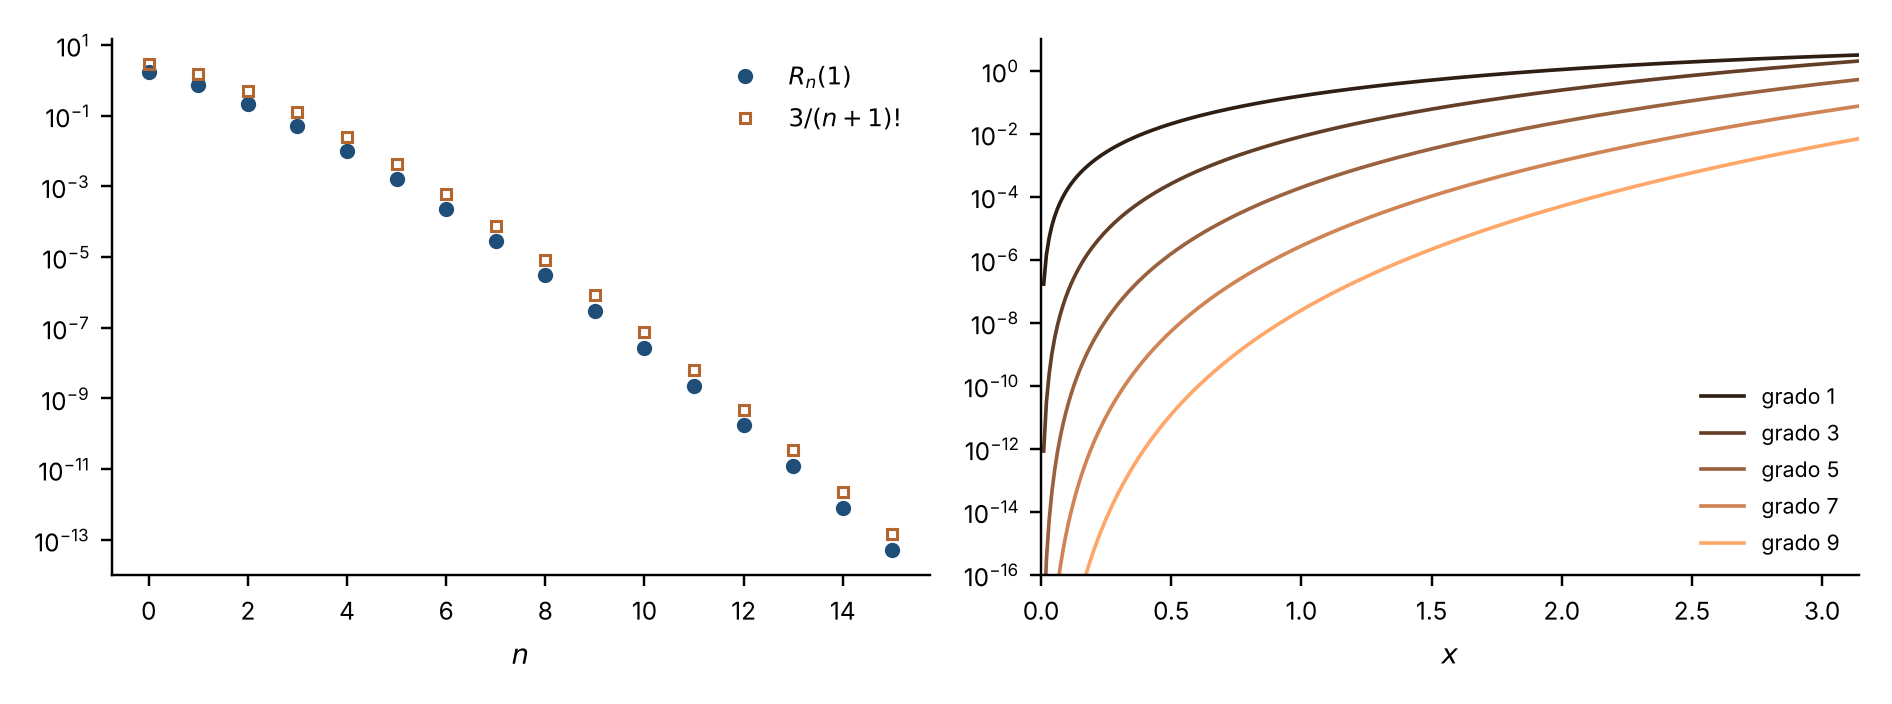
\includegraphics[width=\textwidth]{figure/errore_taylor.png}
\caption{A sinistra: l'errore $R_{n}(1)=e-\sum_{k=0}^{n}\frac1{k!}$ (punti blu) e la stima
$\frac3{(n+1)!}$ (punti rame), in scala logaritmica: la stima segue fedelmente l'errore vero.
A destra: l'errore $\abs{\sen x-T_{2n+1}(x)}$ in $[0,\pi]$ per $2n+1=1,3,5,7,9$; vicino a $0$ i
polinomi di grado alto sono straordinariamente precisi, mentre allontanandosi da $0$
l'errore cresce, pur restando sotto la stima $\frac{x^{2n+3}}{(2n+3)!}$ fornita dal resto di
Lagrange (\texttt{python/fig\_errore\_taylor.py}).}
\label{fig:errore-taylor}
\end{figure}

\begin{idea}[Come calcolano le calcolatrici]
Nessuna calcolatrice usa direttamente lo sviluppo di Taylor per $\sen x$ con $x$ grande:
la \cref{fig:errore-taylor} mostra che l'errore cresce rapidamente allontanandosi dal
centro. Si usa prima la periodicità e la simmetria per ricondurre l'argomento in un
intervallo piccolo, ad esempio $[0,\frac\pi4]$ (\emph{riduzione dell'argomento}), e poi un
polinomio di grado moderato, i cui coefficienti sono spesso leggermente modificati
rispetto a quelli di Taylor per distribuire l'errore uniformemente sull'intervallo
(polinomi di \emph{migliore approssimazione}). Un metodo diverso, che usa soltanto
somme e scorrimenti di cifre, è l'algoritmo CORDIC, ideato nel 1956 da Jack Volder alla
Convair per il calcolatore di navigazione del bombardiere B-58 e poi adottato nelle
prime calcolatrici tascabili.
\end{idea}

\subsection{L'irrazionalità del numero \texorpdfstring{$e$}{e}}

La stima \eqref{eq:stima-e} è così precisa da permettere di dimostrare che $e$ non è un
numero razionale. La dimostrazione, che risale a Fourier, è un piccolo gioiello: si
moltiplica la \eqref{eq:stima-e} per un fattoriale opportuno, in modo da rendere intero
tutto ciò che può esserlo, e si osserva che ciò che resta è un intero strettamente
compreso tra $0$ e $1$.

\begin{teorema}[Irrazionalità di $e$]\label{teo:e-irrazionale}
\index{numero di Nepero!irrazionalità}
Il numero $e$ è irrazionale.
\end{teorema}

\begin{schema}
\Ipotesi{la stima \eqref{eq:stima-e}: $0<e-\sum_{k=0}^{n}\frac1{k!}<\frac3{(n+1)!}$ per ogni $n\ge1$; \
$2<e<3$.}
\Tesi{non esistono interi $p,q\ge1$ con $e=\frac pq$.}
\end{schema}

\begin{strategia}
Ragioniamo per assurdo, supponendo $e=\frac pq$. Moltiplichiamo la \eqref{eq:stima-e}, con
$n=q$, per $q!$: il termine $q!\,e=p\,(q-1)!$ è intero, e lo è anche $q!\sum_{k=0}^{q}\frac1{k!}$, perché
ogni $k!$ con $k\le q$ divide $q!$. Allora anche $q!\,R_{q}(1)$ è un intero; ma la stima del resto
lo pone strettamente tra $0$ e $\frac3{q+1}$, che non supera $1$ se $q\ge2$. Un intero
strettamente compreso tra $0$ e $1$ non esiste.
\end{strategia}

\begin{dimostrazione}
Supponiamo per assurdo che sia $e=\frac pq$ con $p,q$ interi positivi. Poiché $2<e<3$, $e$ non è
intero, e quindi $q\ge2$. Applichiamo la \eqref{eq:stima-e} con $n=q$ e moltiplichiamo per
$q!$:
\[
  0<q!\,e-\sum_{k=0}^{q}\frac{q!}{k!}<\frac{3\,q!}{(q+1)!}=\frac3{q+1} .
\]
Il numero $q!\,e=q!\,\frac pq=p\,(q-1)!$ è intero; anche ogni $\frac{q!}{k!}=(k+1)(k+2)\cdots q$, con
$0\le k\le q$, è intero (per $k=q$ vale $1$). Dunque il numero
$N=q!\,e-\sum_{k=0}^{q}\frac{q!}{k!}$ è intero, e verifica $0<N<\frac3{q+1}\le1$, perché $q\ge2$. Ma non
esistono interi strettamente compresi tra $0$ e $1$: l'assurdo prova la tesi.
\end{dimostrazione}

\subsection{Approfondimento: una tavola dei logaritmi}
\label{subsec:tavola-logaritmi}

Il procedimento del paragrafo funziona male per il logaritmo, se si parte dallo sviluppo
di $\log(1+x)$: per $x=1$ la stima del \cref{sec:taylor-peano} dà soltanto
$\abs{R_{n}(1)}\le\frac1{n+1}$, e per avere $\log2$ con sei decimali esatti occorrerebbero milioni
di termini; per $x>1$, poi, i polinomi si allontanano dalla funzione. Giusti
\cite{giusti} suggerisce invece lo sviluppo di $\log\frac{1+x}{1-x}$, che si ottiene con lo stesso
artificio usato per l'arcotangente nella \cref{prop:sviluppo-arctg}.

\begin{proposizione}[Sviluppo di $\log\frac{1+x}{1-x}$]\label{prop:sviluppo-log-rapporto}
Per ogni intero $n\ge0$ e ogni $x\in(-1,1)$,
\begin{equation}\label{eq:sviluppo-log-rapporto}
\begin{gathered}
  \log\frac{1+x}{1-x}=2\Bigl(x+\frac{x^{3}}3+\frac{x^{5}}5+\dots+\frac{x^{2n+1}}{2n+1}\Bigr)+R(x),\\
  R(x)=2\int_{0}^{x}\frac{t^{2n+2}}{1-t^{2}}\,dt, \qquad
  \abs{R(x)}\le\frac{2\abs x^{2n+3}}{(2n+3)(1-x^{2})} ,
\end{gathered}
\end{equation}
e il resto $R(x)$ ha il segno di $x$.
\end{proposizione}

\begin{schema}
\Ipotesi{$n\ge0$ intero; \ $\abs x<1$.}
\Tesi{la \eqref{eq:sviluppo-log-rapporto}: il resto in forma integrale, la sua stima, e
$R(x)$ dello stesso segno di $x$.}
\end{schema}

\begin{strategia}
La derivata di $\log(1+x)-\log(1-x)$ è $\frac2{1-x^{2}}$, e $\frac1{1-t^{2}}$ è la somma della
progressione geometrica di ragione $t^{2}$, a meno di un resto esplicito. Integrando tra $0$
e $x$ la somma dà il polinomio, e nel resto il denominatore $1-t^{2}$ si minora con il suo
valore nell'estremo $x$.
\end{strategia}

\begin{dimostrazione}
Per $\abs t<1$, la formula della progressione geometrica (\cref{prop:geometrica}) con
ragione $t^{2}\neq1$ dà $\sum_{k=0}^{n}t^{2k}=\frac{1-t^{2n+2}}{1-t^{2}}$, cioè
\[
  \frac1{1-t^{2}}=\sum_{k=0}^{n}t^{2k}+\frac{t^{2n+2}}{1-t^{2}} .
\]
La funzione $g(x)=\log(1+x)-\log(1-x)=\log\frac{1+x}{1-x}$ è derivabile in $(-1,1)$, con
$g'(x)=\frac1{1+x}+\frac1{1-x}=\frac2{1-x^{2}}$ per la \eqref{eq:derivata-log} e la regola della catena,
e $g(0)=0$. Per la formula fondamentale (\cref{teo:formula-fondamentale}), integrando
l'uguaglianza precedente moltiplicata per $2$,
\[
  g(x)=2\int_{0}^{x}\frac{dt}{1-t^{2}}=2\sum_{k=0}^{n}\frac{x^{2k+1}}{2k+1}+R(x) .
\]
Sia $0<x<1$. Per $0\le t\le x$ si ha $1\ge1-t^{2}\ge1-x^{2}>0$, e quindi
$t^{2n+2}\le\frac{t^{2n+2}}{1-t^{2}}\le\frac{t^{2n+2}}{1-x^{2}}$; integrando tra $0$ e $x$, per il
confronto (\cref{teo:confronto-integrali}),
\[
  0<\frac{2x^{2n+3}}{2n+3}\le R(x)\le\frac{2x^{2n+3}}{(2n+3)(1-x^{2})} .
\]
Infine, poiché l'integrando è una funzione pari di $t$, la
sostituzione $t=-u$ mostra che $R(-x)=-R(x)$, e il caso $-1<x<0$ si riconduce al
precedente; per $x=0$ tutto è ovvio.
\end{dimostrazione}

La stima è tanto migliore quanto più $x$ è piccolo, e il quoziente $\frac{1+x}{1-x}$ assume
valori comodi se $x=\frac1{2N+1}$, con $N\in\N$: allora $\frac{1+x}{1-x}=\frac{2N+2}{2N}=\frac{N+1}N$ e
$1-x^{2}=\frac{4N(N+1)}{(2N+1)^{2}}$, sicché
\begin{equation}\label{eq:log-N}
\begin{gathered}
  \log\frac{N+1}N=2\sum_{k=0}^{n}\frac1{(2k+1)\,(2N+1)^{2k+1}}+R, \\
  0<R\le\frac1{2N(N+1)\,(2n+3)\,(2N+1)^{2n+1}} .
\end{gathered}
\end{equation}
Con $N=1$, cioè $x=\frac13$, si ottiene $\log2$: quattro termini ($n=3$) danno
\[
  \log2\simeq2\Bigl(\frac13+\frac1{81}+\frac1{1215}+\frac1{15\,309}\Bigr)=\frac{53\,056}{76\,545}=0{,}6931347\ldots ,
\]
con un errore positivo e inferiore a $\frac1{4\cdot9\cdot3^{7}}=\frac1{78\,732}<1{,}3\cdot10^{-5}$: dunque
$0{,}693134<\log2<0{,}693148$, e $\log2=0{,}6931\ldots$ con quattro decimali esatti; con lo
sviluppo di $\log(1+x)$, per garantire lo stesso errore, la stima richiederebbe quasi
ottantamila termini. Noto $\log2$, si calcolano
$\log3=\log2+\log\frac32$ (con $N=2$), $\log5=2\log2+\log\frac54$ (con $N=4$),
$\log7=\log2+\log3+\log\frac76$ (con $N=6$), e in generale il logaritmo di un primo $p$ dispari
da quelli dei primi minori, perché $p-1$ si scompone in essi, aggiungendo $\log\frac p{p-1}$
con $N=p-1$. Al crescere di $N$ la convergenza diventa sempre più rapida, e i
logaritmi dei primi successivi richiedono pochi termini. Per la proprietà $\log(ab)=\log a+\log b$, dai
logaritmi dei primi si ottengono per somma quelli di tutti gli interi, e dividendo per
$\log10=\log2+\log5$ i logaritmi decimali di Briggs, di cui parla la nota storica che
segue. Il programma costruisce questa piccola tavola con un errore garantito inferiore a
$10^{-13}$ per ciascun termine $\log\frac{N+1}N$, e la confronta con la libreria \texttt{math}.

\needspace{10\baselineskip}
\begin{python}[Una tavola dei logaritmi con errore garantito]
import math
from fractions import Fraction as F

def logN(N, tol=F(1, 10**13)):
    """log((N+1)/N) con x = 1/(2N+1), errore garantito < tol."""
    n = 0
    while F(1, 2*N*(N+1)*(2*n+3)*(2*N+1)**(2*n+1)) >= tol:
        n += 1
    x = F(1, 2*N + 1)
    T = 2 * sum(x**(2*k + 1) / (2*k + 1) for k in range(n + 1))
    return T, n + 1                  # valore e numero di termini

l2, t1 = logN(1)                     # log 2
l32, t2 = logN(2)                    # log 3/2
l54, t4 = logN(4)                    # log 5/4
l76, t6 = logN(6)                    # log 7/6
print("termini per N = 1, 2, 4, 6:", t1, t2, t4, t6)
tavola = {2: l2, 3: l2 + l32, 5: 2*l2 + l54}
tavola[7] = tavola[2] + tavola[3] + l76
for p, v in tavola.items():
    print(f"log {p} = {float(v):.12f}   (math.log: "
          f"{math.log(p):.12f})")
l10 = tavola[2] + tavola[5]
print(f"log10(2) = {float(tavola[2] / l10):.12f}")
\end{python}
\begin{risultato}
termini per N = 1, 2, 4, 6: 13 9 6 6
log 2 = 0.693147180560   (math.log: 0.693147180560)
log 3 = 1.098612288668   (math.log: 1.098612288668)
log 5 = 1.609437912434   (math.log: 1.609437912434)
log 7 = 1.945910149055   (math.log: 1.945910149055)
log10(2) = 0.301029995664
\end{risultato}

Per $N=1$ servono tredici termini, per $N=4$ e $N=6$ ne bastano sei. Gli errori dei
singoli termini si sommano, ma restano dell'ordine di $10^{-13}$: le dodici cifre decimali
stampate coincidono con quelle della libreria. Il valore $\log_{10}2=0{,}30103\ldots$ è quello
che si legge in ogni tavola dei logaritmi decimali.

\begin{notastorica}[Tavole e irrazionalità]
Le prime tavole dei logaritmi furono pubblicate da John Napier nel 1614 (\emph{Mirifici
logarithmorum canonis descriptio}); nel 1624 Henry Briggs pubblicò l'\emph{Arithmetica
logarithmica}, con i logaritmi decimali degli interi da $1$ a $20\,000$ e da $90\,000$ a
$100\,000$, calcolati con quattordici cifre. Quei calcoli, eseguiti a mano con metodi
ingegnosi ma faticosissimi, precedono di decenni la scoperta degli sviluppi in serie.
In seguito le serie fornirono i valori «di appoggio» con grande precisione, come
abbiamo fatto nel \S\ref{subsec:tavola-logaritmi}, mentre il
resto della tavola si completava per interpolazione con il metodo delle differenze
finite: così furono calcolate le grandi tavole francesi dirette da Gaspard de Prony
negli anni Novanta del Settecento, e lo stesso metodo ispirò la macchina alle differenze
di Charles Babbage. Le tavole furono lo strumento quotidiano di astronomi, navigatori e
ingegneri fino all'avvento delle calcolatrici elettroniche. L'irrazionalità
di $e$ fu dimostrata da Eulero nel 1737, mediante lo sviluppo in frazione continua; la
dimostrazione qui riportata, dovuta a Fourier, fu pubblicata nel 1815. Che $e$ sia
addirittura \emph{trascendente}, cioè non sia radice di alcun polinomio a coefficienti
interi, fu dimostrato da Charles Hermite nel 1873.
\end{notastorica}

%% ----------------------------------------------------------------------------
%%  §10.6  Esercizi di riepilogo
%% ----------------------------------------------------------------------------
\section{Esercizi di riepilogo}
\label{sec:esercizi-cap10}

Come nei capitoli precedenti, ogni soluzione è accompagnata da una nota sulla
\emph{scelta logica} che la guida.

\needspace{8\baselineskip}
\subsection*{Sviluppi di Taylor}

\begin{esercizio}[La formula di Machin]\label{es:machin}
Verificare la formula di Machin \eqref{eq:machin}:
$\frac\pi4=4\operatorname{arctg}\frac15-\operatorname{arctg}\frac1{239}$.
\begin{soluzione}
Dividendo le formule di addizione \eqref{eq:addizione-sen} e \eqref{eq:addizione-cos} per
$\cos\alpha\cos\beta$ si ottiene $\tg(\alpha\pm\beta)=\frac{\tg\alpha\pm\tg\beta}{1\mp\tg\alpha\,\tg\beta}$. Sia $\alpha=\operatorname{arctg}\frac15$.
Allora
\[
\begin{gathered}
  \tg2\alpha=\frac{2/5}{1-1/25}=\frac5{12}, \qquad
  \tg4\alpha=\frac{2\cdot5/12}{1-25/144}=\frac{120}{119},\\
  \tg\Bigl(4\alpha-\frac\pi4\Bigr)=\frac{\frac{120}{119}-1}{1+\frac{120}{119}}=\frac1{239} .
\end{gathered}
\]
Poiché $0<\alpha<\frac15$ (si ha $\operatorname{arctg}x<x$ per $x>0$: per la \eqref{eq:sviluppo-arctg}
con $n=0$, il resto $R(x)=-\int_{0}^{x}\frac{t^{2}}{1+t^{2}}\,dt$ è negativo), risulta
$-\frac\pi4<4\alpha-\frac\pi4<\frac45-\frac\pi4<\frac\pi2$; in $(-\frac\pi2,\frac\pi2)$ la tangente è invertibile, e
quindi $4\alpha-\frac\pi4=\operatorname{arctg}\frac1{239}$. \emph{Scelta logica:} un'identità tra
arcotangenti si dimostra calcolando la tangente di entrambi i membri; ma la tangente non
è iniettiva, ed è indispensabile controllare che gli angoli cadano nell'intervallo in cui
essa è invertibile.
\end{soluzione}
\end{esercizio}

\begin{esercizio}\label{es:sviluppo-tangente}
Determinare il polinomio di Taylor di ordine $5$ della funzione $\tg x$ in $x_{0}=0$.
\begin{soluzione}
La funzione $\tg x$ è derivabile infinite volte in $(-\frac\pi2,\frac\pi2)$ ed è dispari; le sue
derivate di ordine pari sono dispari, e quindi nulle in $0$. Il polinomio cercato ha
dunque la forma $x+a_{3}x^{3}+a_{5}x^{5}$ (il coefficiente di $x$ è $\tg'(0)=1$), e
$\tg x=x+a_{3}x^{3}+a_{5}x^{5}+o(x^{5})$. Moltiplicando per
$\cos x=1-\frac{x^{2}}2+\frac{x^{4}}{24}+o(x^{5})$ e usando le regole della \cref{prop:algebra-o},
\[
  \sen x=\tg x\cos x=x+\Bigl(a_{3}-\frac12\Bigr)x^{3}+\Bigl(a_{5}-\frac{a_{3}}2+\frac1{24}\Bigr)x^{5}+o(x^{5}) .
\]
Per l'unicità del polinomio di Taylor (\cref{prop:unicita-taylor}) i coefficienti devono
coincidere con quelli di $\sen x=x-\frac{x^{3}}6+\frac{x^{5}}{120}+o(x^{5})$: $a_{3}-\frac12=-\frac16$, cioè
$a_{3}=\frac13$, e $a_{5}=\frac1{120}+\frac16-\frac1{24}=\frac2{15}$. Dunque
\[
  \tg x=x+\frac{x^{3}}3+\frac{2x^{5}}{15}+o(x^{6}) ,
\]
dove il resto è $o(x^{6})$ perché anche il coefficiente di $x^{6}$ è nullo.
\emph{Scelta logica:} invece di calcolare cinque derivate della tangente, sempre più complicate, si
usa la relazione $\sen x=\tg x\cos x$ tra funzioni di cui conosciamo gli sviluppi, e
l'unicità permette di identificare i coefficienti (\emph{metodo dei coefficienti
indeterminati}).
\end{soluzione}
\end{esercizio}

\begin{esercizio}
Determinare lo sviluppo di Mac Laurin di ordine $5$ di $\arcsen x$.
\begin{soluzione}
Per la \eqref{eq:derivata-arcsen}, $D\arcsen x=(1-x^{2})^{-1/2}$. Dalla \eqref{eq:taylor-potenza}
con $b=-\frac12$, $(1+u)^{-1/2}=1-\frac u2+\frac38\,u^{2}+o(u^{2})$, e con $u=-t^{2}$ (\cref{lem:sostituzione-o})
\[
  \frac1{\sqrt{1-t^{2}}}=1+\frac{t^{2}}2+\frac38\,t^{4}+o(t^{4}) .
\]
Integrando termine a termine tra $0$ e $x$, per la \eqref{eq:integrazione-termine} e poiché
$\arcsen0=0$,
\[
  \arcsen x=x+\frac{x^{3}}6+\frac3{40}\,x^{5}+o(x^{5}) .
\]
\emph{Scelta logica:} come per l'arcotangente, si sviluppa la derivata, che è una
potenza di un binomio, e si integra; il \cref{lem:integrazione-o} garantisce che il resto
integrato è ancora trascurabile, con un ordine in più.
\end{soluzione}
\end{esercizio}

\begin{esercizio}\label{es:derivata-decima}
Sia $f(x)=\sen(x^{2})$. Calcolare $f^{(9)}(0)$ e $f^{(10)}(0)$.
\begin{soluzione}
Dalla \eqref{eq:taylor-sen} con $n=2$ e la sostituzione $t=x^{2}$,
\[
  \sen(x^{2})=x^{2}-\frac{x^{6}}6+\frac{x^{10}}{120}+o(x^{12}) .
\]
Il polinomio a secondo membro, di grado $10$, approssima $f$ con un errore $o(x^{10})$; per
l'unicità è il polinomio di Taylor di ordine $10$, il cui coefficiente di $x^{k}$ è
$\frac{f^{(k)}(0)}{k!}$. Dunque $f^{(9)}(0)=0$ e $\frac{f^{(10)}(0)}{10!}=\frac1{120}$, cioè
$f^{(10)}(0)=\frac{3\,628\,800}{120}=30\,240$. \emph{Scelta logica:} calcolare dieci derivate di
$\sen(x^{2})$ sarebbe proibitivo; l'unicità del polinomio di Taylor permette di leggere le
derivate nei coefficienti di uno sviluppo ottenuto per sostituzione.
\end{soluzione}
\end{esercizio}

\needspace{8\baselineskip}
\subsection*{Limiti e parti principali}

\begin{esercizio}
Calcolare (a) $\displaystyle\lim_{x\to0}\frac{\log(1+x)-\sen x}{x^{2}}$; \
(b) $\displaystyle\lim_{x\to0}\frac{e^{x^{2}}-\cos x-\frac32x^{2}}{x^{4}}$; \
(c) $\displaystyle\lim_{x\to0}\frac{\tg x-\sen x}{x^{3}}$.
\begin{soluzione}
(a) Il denominatore ha ordine $2$: basta sviluppare al secondo ordine.
$\log(1+x)=x-\frac{x^{2}}2+o(x^{2})$ e $\sen x=x+o(x^{2})$, dunque il numeratore è
$-\frac{x^{2}}2+o(x^{2})$ e il limite vale $-\frac12$.

(b) Occorre il quarto ordine. Con $t=x^{2}$ nello sviluppo dell'esponenziale,
$e^{x^{2}}=1+x^{2}+\frac{x^{4}}2+o(x^{4})$; inoltre $\cos x=1-\frac{x^{2}}2+\frac{x^{4}}{24}+o(x^{5})$. Il
numeratore è
$x^{2}+\frac{x^{2}}2-\frac32\,x^{2}+\bigl(\frac12-\frac1{24}\bigr)x^{4}+o(x^{4})=\frac{11}{24}\,x^{4}+o(x^{4})$, e il
limite vale $\frac{11}{24}$.

(c) Per l'\cref{es:sviluppo-tangente}, $\tg x-\sen x=\frac{x^{3}}3+\frac{x^{3}}6+o(x^{4})=\frac{x^{3}}2+o(x^{4})$, e
il limite vale $\frac12$.

\emph{Scelta logica:} l'ordine dello sviluppo è dettato dal denominatore (la sua parte
principale); se i termini del numeratore si elidono fino a quell'ordine, il limite è
zero, altrimenti la \cref{prop:parte-principale} lo fornisce subito.
\end{soluzione}
\end{esercizio}

\begin{esercizio}
Calcolare $\displaystyle\lim_{n\to+\infty}n^{2}\Bigl(1-n\sen\frac1n\Bigr)$.
\begin{soluzione}
Con $x=\frac1n\to0$ il limite è quello di $\frac{1}{x^{2}}\bigl(1-\frac{\sen x}x\bigr)=\frac{x-\sen x}{x^{3}}$. Poiché
$x-\sen x=\frac{x^{3}}6+o(x^{4})$, il limite vale $\frac16$. \emph{Scelta logica:} un limite di
successione che contiene $\frac1n$ in funzioni elementari si riconduce, mediante la
definizione di limite con le successioni, a un limite di funzione per $x\to0$, dove gli
sviluppi di Taylor sono disponibili.
\end{soluzione}
\end{esercizio}

\begin{esercizio}\label{es:verifica-19-30}
Determinare la parte principale, per $x\to0$, di $N(x)=3x^{3}-3x\cos x+\sen3x$, e
dedurre che la funzione dell'\cref{es:limite-taylor-2} è un infinitesimo equivalente a
$\frac{19}{30}\,x$.
\begin{soluzione}
Nell'\cref{es:limite-taylor-2} gli sviluppi fino all'ordine $4$ hanno dato $N(x)=o(x^{4})$.
Aggiungiamo un termine: $\cos x=1-\frac{x^{2}}2+\frac{x^{4}}{24}+o(x^{5})$, quindi
$3x\cos x=3x-\frac32x^{3}+\frac18x^{5}+o(x^{6})$, e
$\sen3x=3x-\frac92x^{3}+\frac{243}{120}x^{5}+o(x^{6})$. Allora
\[
  N(x)=\Bigl(-\frac18+\frac{81}{40}\Bigr)x^{5}+o(x^{6})=\frac{19}{10}\,x^{5}+o(x^{6}) .
\]
Per la \cref{prop:parte-principale} con $p=5$, $q=4$, la funzione $\frac{N(x)}{3x^{4}}$ è
$\frac{19}{30}\,x\,(1+o(1))$. \emph{Scelta logica:} quando tutti i termini fino a un certo ordine si
elidono, il limite è zero; per sapere \emph{come} la funzione tende a zero occorre
spingere lo sviluppo fino al primo termine superstite.
\end{soluzione}
\end{esercizio}

\begin{esercizio}
Determinare l'ordine di infinitesimo e la parte principale di $f(x)=\sen x-x\cos x$ per
$x\to0$, e calcolare $\displaystyle\lim_{x\to0}\frac{\sen x-x\cos x}{x-\sen x}$.
\begin{soluzione}
$\sen x=x-\frac{x^{3}}6+o(x^{4})$ e $x\cos x=x-\frac{x^{3}}2+o(x^{4})$, dunque
$f(x)=\frac{x^{3}}3+o(x^{4})$: $f$ è un infinitesimo di ordine $3$ con parte principale $\frac{x^{3}}3$.
Poiché $x-\sen x=\frac{x^{3}}6+o(x^{4})$, per la \cref{prop:parte-principale} il limite vale
$\frac{1/3}{1/6}=2$. \emph{Scelta logica:} con il teorema di L'Hôpital occorrerebbero più
applicazioni successive, con derivate sempre più lunghe; con gli sviluppi bastano due
righe.
\end{soluzione}
\end{esercizio}

\needspace{8\baselineskip}
\subsection*{Resto e stime}

\begin{esercizio}\label{es:log-disuguaglianza}
Dimostrare che per ogni $x>0$ si ha $x-\frac{x^{2}}2<\log(1+x)<x$.
\begin{soluzione}
Sia $f(x)=\log(1+x)$: $f'(x)=\frac1{1+x}$, $f''(x)=-\frac1{(1+x)^{2}}$, $f'''(x)=\frac2{(1+x)^{3}}$. Per il
\cref{teo:resto-lagrange-generale}, applicato in $(-1,+\infty)$ con $x_{0}=0$, esistono
$x_{1},x_{2}\in(0,x)$ tali che
\[
\begin{aligned}
  \log(1+x)&=x-\frac{x^{2}}{2(1+x_{1})^{2}}<x,\\
  \log(1+x)&=x-\frac{x^{2}}2+\frac{x^{3}}{3(1+x_{2})^{3}}>x-\frac{x^{2}}2 .
\end{aligned}
\]
\emph{Scelta logica:} quando la derivata $f^{(n+1)}$ ha segno costante, il resto di
Lagrange ha segno noto, e la formula di Taylor diventa una disuguaglianza.
\end{soluzione}
\end{esercizio}

\begin{esercizio}
Calcolare $\sqrt{1{,}1}$ con un errore inferiore a $10^{-4}$.
\begin{soluzione}
Sia $f(x)=\sqrt{1+x}$, $x_{0}=0$, $x=\frac1{10}$. Le derivate sono
$f'=\frac12(1+x)^{-1/2}$, $f''=-\frac14(1+x)^{-3/2}$, $f'''=\frac38(1+x)^{-5/2}$. Con $n=1$ la stima
\eqref{eq:stima-resto} dà $\abs{R_{1}}\le\frac14\cdot\frac{10^{-2}}2=1{,}25\cdot10^{-3}$, insufficiente. Con
$n=2$, poiché $0<f'''\le\frac38$ in $[0,\frac1{10}]$,
\[
  0<R_{2}\Bigl(\frac1{10}\Bigr)\le\frac38\cdot\frac{10^{-3}}{6}=6{,}25\cdot10^{-5}<10^{-4} ,
\]
e $T_{2}(\frac1{10})=1+\frac1{20}-\frac1{800}=1{,}04875$. Dunque
$1{,}04875<\sqrt{1{,}1}\le1{,}0488125$ (il valore esatto è $1{,}0488088\ldots$).
\emph{Scelta logica:} si aumenta $n$ finché la stima del resto scende sotto la precisione richiesta;
il segno di $f'''$ dice inoltre da che parte sta l'errore.
\end{soluzione}
\end{esercizio}

\begin{esercizio}[L'integrale della campana di Gauss]\label{es:integrale-gauss-taylor}
Calcolare $\int_{0}^{1}e^{-x^{2}}\,dx$ con un errore inferiore a $10^{-5}$, e confrontare il risultato
con le stime dell'\cref{es:stima-gaussiana}.
\begin{soluzione}
Per il \cref{teo:resto-lagrange} applicato a $g(t)=e^{-t}$ con centro $0$, per ogni $t>0$
esiste $\tau\in(0,t)$ tale che
\[
  e^{-t}=\sum_{k=0}^{n}\frac{(-t)^{k}}{k!}+R_{n}(t), \qquad R_{n}(t)=(-1)^{n+1}\frac{e^{-\tau}}{(n+1)!}\,t^{n+1} ;
\]
dunque $\abs{R_{n}(t)}\le\frac{t^{n+1}}{(n+1)!}$, e $R_{n}(t)$ ha il segno di $(-1)^{n+1}$. Con $t=x^{2}$ la
funzione $R_{n}(x^{2})$, differenza di funzioni continue, è integrabile in $[0,1]$, e per
la linearità e il confronto (\cref{teo:confronto-integrali,teo:valore-assoluto})
\[
\begin{gathered}
  \int_{0}^{1}e^{-x^{2}}dx=\sum_{k=0}^{n}\frac{(-1)^{k}}{k!\,(2k+1)}+E_{n},\\
  \abs{E_{n}}\le\int_{0}^{1}\frac{x^{2n+2}}{(n+1)!}\,dx=\frac1{(n+1)!\,(2n+3)} .
\end{gathered}
\]
Per $n=6$ la stima vale $\frac1{75\,600}\approx1{,}3\cdot10^{-5}$, insufficiente; per $n=7$ vale
$\frac1{685\,440}<1{,}5\cdot10^{-6}$, e inoltre $E_{7}\ge0$, perché $R_{7}\ge0$. Dunque
\[
\begin{aligned}
  \int_{0}^{1}e^{-x^{2}}dx&\simeq1-\frac13+\frac1{10}-\frac1{42}+\frac1{216}-\frac1{1320}
  +\frac1{9360}-\frac1{75\,600}\\
  &=0{,}7468228\ldots
\end{aligned}
\]
per difetto, con un errore inferiore a $1{,}5\cdot10^{-6}$: $0{,}7468228<\int_{0}^{1}e^{-x^{2}}dx<0{,}7468243$.
Otto termini bastano dove le somme integrali dell'\cref{es:stima-gaussiana}, con
$10\,000$ suddivisioni, lasciano un'incertezza di $6\cdot10^{-5}$. \emph{Scelta logica:} se la
funzione integranda non ha una primitiva elementare, la si sostituisce con un polinomio
di Taylor, che si integra esattamente; la stima del resto, integrata, certifica
l'errore.
\end{soluzione}
\end{esercizio}

\begin{esercizio}[Freccia dell'ala con portanza ellittica]\label{es:freccia-ellittica}
Con le notazioni del \cref{sec:applicazioni-integrali} e della \cref{prop:freccia}, sia
$T(y)=\int_{y}^{s}l$ il taglio (da non confondere con un polinomio di Taylor). Dimostrare
che
\[
  \int_{0}^{s}(s-t)M(t)\,dt=\frac{s^{2}}2M(0)-\frac{s^{3}}6T(0)+\frac16\int_{0}^{s}(s-t)^{3}l(t)\,dt ,
\]
e dedurne che per la distribuzione ellittica $l(y)=l_{0}\sqrt{1-(y/s)^{2}}$ la freccia
all'estremità vale $v(s)=\frac{l_{0}s^{4}}{EI}\bigl(\frac\pi{32}-\frac1{45}\bigr)$, cioè
$1-\frac{32}{45\pi}\approx0{,}774$ volte quella dovuta a un carico uniforme con la stessa portanza
totale.
\begin{soluzione}
Si integra per parti due volte, usando $M'=-T$, $T'=-l$ e $M(s)=T(s)=0$
(\cref{prop:taglio-momento}). Con la primitiva $-\frac{(s-t)^{2}}2$ di $s-t$,
\[
\begin{aligned}
  \int_{0}^{s}(s-t)M\,dt&=\Bigl[-\frac{(s-t)^{2}}2M\Bigr]_{0}^{s}-\int_{0}^{s}\frac{(s-t)^{2}}2\,T\,dt\\
  &=\frac{s^{2}}2M(0)-\int_{0}^{s}\frac{(s-t)^{2}}2\,T\,dt ;
\end{aligned}
\]
con la primitiva $-\frac{(s-t)^{3}}6$ di $\frac{(s-t)^{2}}2$,
$\int_{0}^{s}\frac{(s-t)^{2}}2T\,dt=\frac{s^{3}}6T(0)-\frac16\int_{0}^{s}(s-t)^{3}l\,dt$, e la formula segue.
Per la distribuzione ellittica, dall'\cref{es:taglio-ellittico}, $M(0)=\frac{l_{0}s^{2}}3$ e
$T(0)=\frac\pi4l_{0}s$; con $t=sw$,
$\int_{0}^{s}(s-t)^{3}l\,dt=l_{0}s^{4}\int_{0}^{1}(1-w)^{3}\sqrt{1-w^{2}}\,dw$. Sviluppando il cubo e usando
\[
\begin{gathered}
  \int_{0}^{1}\!\sqrt{1-w^{2}}\,dw=\frac\pi4, \qquad \int_{0}^{1}\!w\sqrt{1-w^{2}}\,dw=\frac13,\\
  \int_{0}^{1}\!w^{2}\sqrt{1-w^{2}}\,dw=\frac\pi{16}, \qquad \int_{0}^{1}\!w^{3}\sqrt{1-w^{2}}\,dw=\frac2{15}
\end{gathered}
\]
(il secondo e il quarto con $u=1-w^{2}$, il terzo con $w=\sen\theta$), si trova
$\int_{0}^{1}(1-w)^{3}\sqrt{1-w^{2}}\,dw=\frac\pi4-1+\frac{3\pi}{16}-\frac2{15}=\frac{7\pi}{16}-\frac{17}{15}$. Allora
\[
  EI\,v(s)=l_{0}s^{4}\Bigl[\frac16-\frac\pi{24}+\frac16\Bigl(\frac{7\pi}{16}-\frac{17}{15}\Bigr)\Bigr]
  =l_{0}s^{4}\Bigl(\frac\pi{32}-\frac1{45}\Bigr) .
\]
Con $l_{0}=\frac4\pi\cdot\frac Wb$ e, per il carico uniforme $l=\frac Wb$, $EI\,v(s)=\frac{W}{b}\frac{s^{4}}8$, il
rapporto è $\frac{32}\pi\bigl(\frac\pi{32}-\frac1{45}\bigr)=1-\frac{32}{45\pi}\approx0{,}7736$, in accordo con il
calcolo numerico del \cref{sec:resto-integrale}. \emph{Scelta logica:} ogni integrazione
per parti trasferisce una derivata dal peso polinomiale alle grandezze della trave,
scendendo da $M$ a $T$ e da $T$ al carico $l$, che è noto esplicitamente; i termini di
bordo all'estremità libera si annullano perché lì taglio e momento sono nulli.
\end{soluzione}
\end{esercizio}

\needspace{8\baselineskip}
\subsection*{Taylor e calcolo numerico}

\begin{esercizio}[L'errore delle differenze finite]\label{es:errore-differenze}
Sia $f$ di classe $C^{3}$ in un intervallo contenente $[x-h,x+h]$, con $h>0$, e siano
$M_{2}$ e $M_{3}$ i massimi di $\abs{f''}$ e di $\abs{f'''}$ in quell'intervallo. Dimostrare che
\[
\begin{aligned}
  \Bigl|\frac{f(x+h)-f(x)}h-f'(x)\Bigr|&\le\frac{M_{2}}2\,h ,\\
  \Bigl|\frac{f(x+h)-f(x-h)}{2h}-f'(x)\Bigr|&\le\frac{M_{3}}6\,h^{2} .
\end{aligned}
\]
\begin{soluzione}
Per il \cref{teo:resto-lagrange} con $n=1$, $f(x+h)=f(x)+f'(x)h+\frac{f''(\xi)}2h^{2}$ con $\xi$
tra $x$ e $x+h$: dividendo per $h$ si ottiene la prima stima. Con $n=2$,
\[
  f(x\pm h)=f(x)\pm f'(x)h+\frac{f''(x)}2h^{2}\pm\frac{f'''(\xi_{\pm})}6h^{3} ,
\]
con $\xi_{+}\in(x,x+h)$ e $\xi_{-}\in(x-h,x)$. Sottraendo, i termini con $f(x)$ e con $f''(x)$ si
elidono:
\[
  \frac{f(x+h)-f(x-h)}{2h}-f'(x)=\frac{f'''(\xi_{+})+f'''(\xi_{-})}{12}\,h^{2} ,
\]
che in valore assoluto non supera $\frac{2M_{3}}{12}h^{2}=\frac{M_{3}}6h^{2}$. Sono le leggi osservate
numericamente nel \cref{cap:derivate}: dividendo $h$ per $10$, l'errore della differenza in
avanti si divide per $10$, quello della differenza centrata per $100$. \emph{Scelta
logica:} la simmetria della differenza centrata fa elidere il termine di secondo ordine;
per vederlo basta scrivere la formula di Taylor nei due punti $x\pm h$ e sottrarre.
\end{soluzione}
\end{esercizio}

\begin{esercizio}[La convergenza quadratica del metodo di Newton]\label{es:newton-quadratico}
Sia $f$ di classe $C^{2}$ in un intervallo $I$ contenente una radice $r$ di $f$, con $f'\neq0$
in $I$, e sia $x_{n+1}=x_{n}-\frac{f(x_{n})}{f'(x_{n})}$ la successione del metodo di Newton
(\cref{es:newton}). Dimostrare che, se $x_{n}\in I$, esiste $\xi$ tra $x_{n}$ e $r$ tale che
\[
  x_{n+1}-r=\frac{f''(\xi)}{2f'(x_{n})}\,(x_{n}-r)^{2} ,
\]
e dedurne che, se $\abs{f''}\le M_{2}$ e $\abs{f'}\ge m_{1}>0$ in $I$, l'errore verifica
$\abs{x_{n+1}-r}\le\frac{M_{2}}{2m_{1}}\abs{x_{n}-r}^{2}$.
\begin{soluzione}
Per il \cref{teo:resto-lagrange} con centro $x_{n}$, calcolato in $r$,
$0=f(r)=f(x_{n})+f'(x_{n})(r-x_{n})+\frac{f''(\xi)}2(r-x_{n})^{2}$. Dividendo per $f'(x_{n})$ e
ricordando che $\frac{f(x_{n})}{f'(x_{n})}=x_{n}-x_{n+1}$,
\[
  0=x_{n}-x_{n+1}+r-x_{n}+\frac{f''(\xi)}{2f'(x_{n})}(r-x_{n})^{2} ,
\]
che è la tesi. La stima segue maggiorando $\abs{f''(\xi)}$ con $M_{2}$ e minorando $\abs{f'(x_{n})}$
con $m_{1}$. Se l'errore è dell'ordine di $10^{-k}$, al passo successivo è dell'ordine di
$10^{-2k}$ (a meno della costante $\frac{M_{2}}{2m_{1}}$): il numero di cifre esatte all'incirca
raddoppia a ogni iterazione, come si era osservato nel \cref{cap:derivate}. \emph{Scelta
logica:} l'errore del metodo di Newton è il resto della formula di Taylor di ordine $1$,
perché il metodo sostituisce $f$ con la sua retta tangente; il resto di Lagrange lo
rende esplicito.
\end{soluzione}
\end{esercizio}

\needspace{8\baselineskip}
\subsection*{Applicazioni aeronautiche}

\begin{esercizio}[Arco e corda di cerchio massimo]
Due aeroporti distano $s=1000$~km lungo un cerchio massimo della Terra ($R=6371$~km).
Stimare di quanto la corda che li congiunge (la distanza in linea retta) è più corta
dell'arco, e controllare l'errore della stima.
\begin{soluzione}
L'angolo al centro è $\frac sR$, e la corda vale $2R\sen\frac s{2R}$. Posto $u=\frac s{2R}$, la
differenza è $s-2R\sen u=2R(u-\sen u)$. Per il \cref{teo:resto-lagrange} con $n=4$
($T_{4}(u)=u-\frac{u^{3}}6$, e $\abs{\sen^{(5)}}=\abs{\cos}\le1$),
$u-\sen u=\frac{u^{3}}6-R_{4}(u)$ con $\abs{R_{4}(u)}\le\frac{u^{5}}{120}$. Dunque
\[
  s-2R\sen\frac s{2R}=\frac{s^{3}}{24R^{2}}+E, \qquad
  \abs E\le2R\,\frac{u^{5}}{120}=\frac{s^{5}}{1920R^{4}} .
\]
Numericamente $\frac{s^{3}}{24R^{2}}\approx1{,}0265$~km e $\abs E\le3{,}2\cdot10^{-4}$~km: la corda è più corta
dell'arco di circa $1026$~m, con un'incertezza di qualche decimetro.
\emph{Scelta logica:} la differenza di due quantità quasi uguali si calcola sviluppando,
in modo che la cancellazione avvenga «sulla carta» e non nel calcolo numerico; il resto
di Lagrange certifica l'accuratezza della stima.
\end{soluzione}
\end{esercizio}

\begin{esercizio}[L'orizzonte, al secondo ordine]\label{es:orizzonte-secondo-ordine}
Con le notazioni del riquadro sulla distanza dell'orizzonte (\cref{sec:taylor-peano}),
dimostrare che per $h\to0$
\[
  d=R\arccos\frac R{R+h}=\sqrt{2Rh}\,\Bigl(1-\frac{5h}{12R}+o(h)\Bigr) ,
\]
e spiegare la colonna «differenza» della tabella prodotta dal programma.
\begin{soluzione}
Posto $\varepsilon=\frac hR$, l'angolo $\vartheta$ verifica $\cos\vartheta=\frac1{1+\varepsilon}$, e quindi
$1-\cos\vartheta=\frac\varepsilon{1+\varepsilon}=\varepsilon-\varepsilon^{2}+o(\varepsilon^{2})$. D'altra parte
$1-\cos\vartheta=\frac{\vartheta^{2}}2-\frac{\vartheta^{4}}{24}+o(\vartheta^{5})$. Al primo ordine si trova
$\vartheta^{2}=2\varepsilon+o(\varepsilon)$, dunque $\vartheta^{4}=4\varepsilon^{2}+o(\varepsilon^{2})$ e, poiché
$\frac{\vartheta^{5}}{\varepsilon^{2}}\to0$, anche $o(\vartheta^{5})=o(\varepsilon^{2})$. Allora
\[
  \frac{\vartheta^{2}}2=\varepsilon-\varepsilon^{2}+\frac{\varepsilon^{2}}6+o(\varepsilon^{2}) ,
  \qquad\text{cioè}\qquad
  \vartheta^{2}=2\varepsilon\Bigl(1-\frac56\,\varepsilon+o(\varepsilon)\Bigr) ,
\]
e, con lo sviluppo $(1+u)^{1/2}=1+\frac u2+o(u)$, $\vartheta=\sqrt{2\varepsilon}\,\bigl(1-\frac5{12}\,\varepsilon+o(\varepsilon)\bigr)$.
Moltiplicando per $R$ si ottiene la tesi. L'approssimazione $\sqrt{2Rh}$ \emph{sovrastima}
dunque la distanza, di circa $\sqrt{2Rh}\,\frac{5h}{12R}$: per $h=10$~km sono
$356{,}96\cdot\frac{50}{76\,452}\approx0{,}233$~km, proprio la differenza calcolata dal programma.
\emph{Scelta logica:} per conoscere l'errore di un'approssimazione «al primo ordine» si
spinge lo sviluppo all'ordine successivo; qui l'incognita $\vartheta$ compare in uno
sviluppo, e la si ricava per approssimazioni successive.
\end{soluzione}
\end{esercizio}

\begin{esercizio}[La correzione di compressibilità del tubo di Pitot]
\label{es:compressibilita}
In un flusso subsonico di un gas perfetto con $\gamma=1{,}4$, la pressione totale $p_{0}$
misurata dal tubo di Pitot e la pressione statica $p$ sono legate al numero di Mach $M$
dalla relazione isentropica $\frac{p_{0}}p=\bigl(1+\frac{\gamma-1}2M^{2}\bigr)^{\gamma/(\gamma-1)}=\bigl(1+\frac{M^{2}}5\bigr)^{7/2}$,
mentre la pressione dinamica vale $q=\frac\gamma2pM^{2}=0{,}7\,pM^{2}$. Dimostrare che
\[
  \frac{p_{0}-p}{q}=1+\frac{M^{2}}4+\frac{M^{4}}{40}+o(M^{4}) \qquad (M\to0) ,
\]
e valutare l'errore che si commette usando l'equazione di Bernoulli incomprimibile
$p_{0}-p=q$ a $M=0{,}3$.
\begin{soluzione}
Dalla \eqref{eq:taylor-potenza} con $b=\frac72$,
$(1+u)^{7/2}=1+\frac72u+\frac{35}8u^{2}+\frac{35}{16}u^{3}+o(u^{3})$, e con $u=\frac{M^{2}}5$
(\cref{lem:sostituzione-o} e \cref{prop:algebra-o})
\[
  \frac{p_{0}}p=1+0{,}7\,M^{2}+0{,}175\,M^{4}+0{,}0175\,M^{6}+o(M^{6}) .
\]
Sottraendo $1$ e dividendo per $\frac qp=0{,}7\,M^{2}$, per la \eqref{eq:o-quoziente},
$\frac{p_{0}-p}q=1+0{,}25\,M^{2}+0{,}025\,M^{4}+o(M^{4})$. A $M=0{,}3$ la correzione vale
$\frac{0{,}09}4+\frac{0{,}0081}{40}\approx0{,}0227$: a velocità assegnata, l'equazione di Bernoulli
incomprimibile sottostima la pressione di impatto $p_{0}-p$ di circa il $2{,}3\%$.
Viceversa, se dalla pressione di impatto misurata si deduce la velocità con l'equazione
incomprimibile, la si \emph{sovrastima}; poiché la velocità è proporzionale alla radice
di $p_{0}-p$, l'errore è circa la metà, l'$1{,}1\%$.
Il risultato è coerente con la regola pratica secondo cui la compressibilità è
trascurabile fino a $M\approx0{,}3$ (regola che di solito si giustifica con la variazione
relativa di densità, circa $\frac{M^{2}}2\approx4{,}5\%$ a $M=0{,}3$).
\emph{Scelta logica:} lo sviluppo del binomio con esponente reale trasforma
una relazione esatta ma poco trasparente in una correzione «a potenze di $M^{2}$», il cui
primo termine misura l'effetto della compressibilità.
\end{soluzione}
\end{esercizio}

\begin{python}[Verifica degli esercizi]
import math
import sympy as sp

x, M = sp.symbols('x M')
print(sp.series(sp.tan(x), x, 0, 7))
print(sp.series(sp.asin(x), x, 0, 7))
print(sp.diff(sp.sin(x**2), x, 10).subs(x, 0))
for e in (sp.log(1 + x) - sp.sin(x),
          sp.exp(x**2) - sp.cos(x) - sp.Rational(3, 2) * x**2,
          sp.tan(x) - sp.sin(x)):
    k = sp.Poly(sp.series(e, x, 0, 6).removeO(), x).monoms()[-1][0]
    print(f"limite = {sp.limit(e / x**k, x, 0)}  (ordine {k})")

R, s = 6371.0, 1000.0
print(f"arco - corda = {1000 * (s - 2*R*math.sin(s/(2*R))):.2f} m"
      f",  s^3/(24R^2) = {1000 * s**3 / (24 * R**2):.2f} m")

r = sp.Rational
esatto = ((1 + M**2 / 5)**r(7, 2) - 1) / (r(7, 10) * M**2)
print(sp.series(esatto, M, 0, 6))
for m in (0.1, 0.3, 0.5, 0.7):
    serie = 1 + m**2 / 4 + m**4 / 40
    print(f"M = {m}:  esatto {float(esatto.subs(M, m)):.5f}"
          f"   serie {serie:.5f}")
\end{python}
\begin{risultato}
x + x**3/3 + 2*x**5/15 + O(x**7)
x + x**3/6 + 3*x**5/40 + O(x**7)
30240
limite = -1/2  (ordine 2)
limite = 11/24  (ordine 4)
limite = 1/2  (ordine 3)
arco - corda = 1026.22 m,  s^3/(24R^2) = 1026.53 m
1 + M**2/4 + M**4/40 + O(M**6)
M = 0.1:  esatto 1.00250   serie 1.00250
M = 0.3:  esatto 1.02270   serie 1.02270
M = 0.5:  esatto 1.06407   serie 1.06406
M = 0.7:  esatto 1.12858   serie 1.12850
\end{risultato}

%% ----------------------------------------------------------------------------
%%  §10.7  Punti fondamentali del capitolo
%% ----------------------------------------------------------------------------
\section{Punti fondamentali del capitolo}
\label{sec:sintesi-cap10}

Il capitolo ha completato la formula di Taylor in due direzioni. Il resto di Peano,
manipolato con l'algebra degli o piccoli, descrive l'errore \emph{vicino} al punto
iniziale ed è lo strumento più efficace per i limiti; il resto integrale e quello di
Lagrange ne danno invece il \emph{valore} per un $x$ fissato, e trasformano
l'approssimazione con un polinomio in un calcolo con precisione garantita.

\begin{puntichiave}
\item \textbf{Il polinomio di Taylor senza derivate.} Un polinomio di grado $\le n$
coincide con il proprio sviluppo di ordine $n$ in ogni punto
(\cref{prop:polinomio-sviluppo}). Se $f$ è derivabile $n$ volte in $x_{0}$, qualunque
polinomio di grado $\le n$ che differisce da $f$ per un $o\bigl((x-x_{0})^{n}\bigr)$ è il
polinomio di Taylor (\cref{prop:unicita-taylor}): gli sviluppi si possono ottenere con
qualunque procedimento, senza calcolare derivate.
\item \textbf{Sostituzione e integrazione.} Se $g(t)=o(t^{m})$ per $t\to0$, e $\varphi(x)\to0$
con $\varphi(x)\neq0$ per $x\neq x_{0}$, allora $g(\varphi(x))=o(\varphi(x)^{m})$
(\cref{lem:sostituzione-o}). Se inoltre $g$ è continua vicino a $0$, allora
$\int_{0}^{x}g(t)\,dt=o(x^{m+1})$
(\cref{lem:integrazione-o}): lo sviluppo di una derivata continua si integra termine a
termine. Derivare termine a termine, invece, non è lecito in generale.
\item \textbf{L'arcotangente.} Per ogni $n\ge0$ e ogni $x\in\R$,
$\operatorname{arctg}x=\sum_{k=0}^{n}(-1)^{k}\frac{x^{2k+1}}{2k+1}+R(x)$ con
$\abs{R(x)}\le\frac{\abs x^{2n+3}}{2n+3}$ (\cref{prop:sviluppo-arctg}). Per $\abs x\le1$ il resto
tende a zero (serie di Leibniz, formula di Machin per le cifre di $\pi$); per $\abs x>1$ i
polinomi si allontanano dalla funzione (\cref{fig:taylor-arctg}).
\item \textbf{L'algebra degli o piccoli.} Le uguaglianze con gli o piccoli si leggono
da sinistra a destra (\cref{prop:algebra-o}): ad esempio $x^{m}\,o(x^{n})=o(x^{m+n})$,
$o(x^{m})\,o(x^{n})=o(x^{m+n})$ e $\frac{o(x^{n})}{x^{m}}=o(x^{n-m})$ per $m\le n$. Errore tipico:
$o(x^{n})-o(x^{n})$ non è zero, ma ancora $o(x^{n})$, e un rapporto $\frac{o(x^{n})}{o(x^{n})}$
non ha un significato preciso.
\item \textbf{Parti principali.} Se $\varphi(x)=a\,x^{k}+o(x^{k})$ con $a\neq0$ e $k,m\ge1$, allora
$\varphi(x)^{m}=a^{m}x^{km}+o(x^{km})$ e $o(\varphi(x)^{m})=o(x^{km})$
(\cref{cor:o-composto}), il che permette di comporre gli sviluppi. Se
$f(x)=a\,x^{p}+o(x^{p})$ e $g(x)=b\,x^{q}+o(x^{q})$ con $a,b\neq0$, allora
$\frac{f(x)}{g(x)}=\frac ab\,x^{p-q}\bigl(1+o(1)\bigr)$ (\cref{prop:parte-principale}): nel limite
di un rapporto numeratore e denominatore si sostituiscono con le loro parti principali
(\cref{def:parte-principale}).
\item \textbf{Fino a che ordine sviluppare.} L'ordine è dettato dalla parte principale
del denominatore, e il numeratore va sviluppato fino al primo termine che non si elide.
Uno sviluppo troppo corto lascia una forma indeterminata come $\frac{o(x^{2})}{x^{3}}$
(\cref{es:limite-taylor-1}); se tutto si elide fino all'ordine del denominatore, il
limite è zero (\cref{es:limite-taylor-2}).
\item \textbf{Taylor contro la cancellazione.} Nel calcolo in virgola mobile la
differenza di due numeri grandi e quasi uguali perde cifre significative; lo sviluppo di
Taylor esegue la sottrazione «sulla carta» ed è il rimedio sistematico
(\cref{fig:cancellazione}).
\item \textbf{Il resto integrale.} Se $f$ è di classe $C^{n+1}$ in $[a,b]$ e
$x_{0},x\in[a,b]$, allora $R_{n}(x)=\int_{x_{0}}^{x}\frac{(x-t)^{n}}{n!}f^{(n+1)}(t)\,dt$
(\cref{teo:resto-integrale}), formula che si dimostra per induzione integrando per parti.
Ad esempio, poiché le derivate di $e^{x}$ sono positive, $e^{x}$ supera tutti i suoi
polinomi di Taylor per $x>0$ (\cref{es:exp-maggiore-taylor}).
\item \textbf{La freccia di un'ala a sbalzo.} Se il carico $l$ è continuo, $EI$ è
costante e $v$, di classe $C^{2}$, verifica $v''=\frac M{EI}$ con $v(0)=v'(0)=0$, la
formula di Taylor di ordine $1$ con resto integrale dà
$v(y)=\frac1{EI}\int_{0}^{y}(y-t)M(t)\,dt$ (\cref{prop:freccia}). Con un carico uniforme la
freccia all'estremità vale $\frac{l\,s^{4}}{8EI}$; a parità di portanza totale, la
distribuzione ellittica la riduce a circa $0{,}774$ volte questo valore
(\cref{es:freccia-ellittica}).
\item \textbf{Il resto di Lagrange.} Se $f$ è di classe $C^{n+1}$ in $[a,b]\ni x_{0}$, per
ogni $x\in[a,b]$ esiste $x_{1}$ tra $x_{0}$ e $x$ con
$R_{n}(x)=\frac{f^{(n+1)}(x_{1})}{(n+1)!}\,{(x-x_{0})}^{n+1}$
(\cref{teo:resto-lagrange}), grazie al teorema della media pesata
(\cref{lem:media-pesata}). Basta in realtà che $f$ sia derivabile $n+1$ volte in un
intervallo aperto (\cref{teo:resto-lagrange-generale}); per $n=0$ si ritrova il teorema
di Lagrange. Il punto $x_{1}$ non è noto, e dipende sia da $x$ sia da $n$.
\item \textbf{La stima del resto.} Se $f$ è di classe $C^{n+1}$ in $[a,b]\ni x_{0}$ e
$M_{n+1}$ è il massimo di $\abs{f^{(n+1)}}$ in $[a,b]$, allora
$\abs{R_{n}(x)}\le M_{n+1}\frac{\abs{x-x_{0}}^{n+1}}{(n+1)!}$ (\cref{cor:stima-resto}).
Per calcolare una funzione con precisione prefissata si sceglie $x_{0}$ vicino a $x$, con
derivate note, e si aumenta $n$ finché la stima scende sotto la tolleranza; per il seno
conviene leggere $x-\frac{x^{3}}6$ come polinomio di ordine $4$, e non $3$
(\cref{es:sen-un-decimo}).
\item \textbf{Il segno del resto.} Se $f^{(n+1)}$ ha segno costante, anche il resto di
Lagrange lo ha, e la formula di Taylor diventa una disuguaglianza: ad esempio
$x-\frac{x^{2}}2<\log(1+x)<x$ per $x>0$ (\cref{es:log-disuguaglianza}), e
$\abs{\sen\varphi-\varphi}\le\frac{\abs\varphi^{3}}6$ per ogni $\varphi$, che controlla
l'approssimazione dei piccoli angoli (\cref{es:piccoli-angoli-stima}).
\item \textbf{Il numero $e$.} Per ogni $n\ge0$ vale
$0<e-\sum_{k=0}^{n}\frac1{k!}<\frac3{(n+1)!}$ (\cref{es:calcolo-e}): undici termini danno sette
decimali esatti. Moltiplicando questa stima per $q!$ si dimostra che $e$ è irrazionale
(\cref{teo:e-irrazionale}).
\item \textbf{Applicazioni aeronautiche.} La distanza dell'orizzonte da una quota $h$ è
$d=\sqrt{2Rh}\,\bigl(1-\frac{5h}{12R}+o(h)\bigr)$: la formula $\sqrt{2Rh}$ la sovrastima
leggermente (\cref{es:orizzonte-secondo-ordine}). Per il tubo di Pitot, con $\gamma=1{,}4$,
$\frac{p_{0}-p}{q}=1+\frac{M^{2}}4+\frac{M^{4}}{40}+o(M^{4})$, e a $M=0{,}3$ l'equazione di
Bernoulli incomprimibile sottostima la pressione d'impatto di circa il $2{,}3\%$
(\cref{es:compressibilita}).
\end{puntichiave}

\paragraph{Il filo del discorso.} Le stime del resto hanno mostrato che per alcune
funzioni e alcuni valori di $x$ il resto $R_{n}(x)$ tende a zero per $n\to+\infty$ (per
l'arcotangente con $\abs x\le1$, per l'esponenziale in $x=1$), mentre per l'arcotangente
con $\abs x>1$ non tende a zero.
Resta aperta la domanda di fondo: che senso dare a una «somma di infiniti termini», e
quando la somma dei termini dello sviluppo restituisce proprio $f(x)$? Il
\cref{cap:serie} risponde con la teoria delle serie numeriche e, nella sua appendice,
con le serie di Taylor e i criteri di sviluppabilità (\cref{teo:sviluppabilita}).

